\documentclass[a4paper,12pt]{article}[abntex2]
\bibliographystyle{abntex2-alf}
\usepackage{siunitx} % Fornece suporte para a tipografia de unidades do Sistema Internacional e formatação de números
\usepackage{booktabs} % Melhora a qualidade das tabelas
\usepackage{tabularx} % Permite tabelas com larguras de colunas ajustáveis
\usepackage{graphicx} % Suporte para inclusão de imagens
\usepackage{newtxtext} % Substitui a fonte padrão pela Times Roman
\usepackage{ragged2e} % Justificação de texto melhorada
\usepackage{setspace} % Controle do espaçamento entre linhas
\usepackage[a4paper, left=3.0cm, top=3.0cm, bottom=2.0cm, rigH=2.0cm]{geometry} % Personalização das margens do documento
\usepackage{lipsum} % Geração de texto dummy 'Lorem Ipsum'
\usepackage{fancyhdr} % Customização de cabeçalhos e rodapés
\usepackage{titlesec} % Personalização dos títulos de seções
\usepackage[portuguese]{babel} % Adaptação para o português (nomes e hifenização
\usepackage{hyperref} % Suporte a hiperlinks
\usepackage{indentfirst} % Indentação do primeiro parágrafo das seções
\sisetup{
  output-decimal-marker = {,},
  inter-unit-product = \ensuremath{{}\cdot{}},
  per-mode = symbol
}
\DeclareSIUnit{\real}{R\$}
\newcommand{\real}[1]{R\$#1}
\usepackage{float} % Melhor controle sobre o posicionamento de figuras e tabelas
\usepackage{footnotehyper} % Notas de rodapé clicáveis em combinação com hyperref
\hypersetup{
    colorlinks=true,
    linkcolor=black,
    filecolor=magenta,      
    urlcolor=cyan,
    citecolor=black,        
    pdfborder={0 0 0},
}
\usepackage[normalem]{ulem} % Permite o uso de diferentes tipos de sublinhados sem alterar o \emph{}
\makeatletter
\def\@pdfborder{0 0 0} % Remove a borda dos links
\def\@pdfborderstyle{/S/U/W 1} % Estilo da borda dos links
\makeatother
\onehalfspacing

\begin{document}

\begin{titlepage}
    \centering
    \vspace*{1cm}
    \Large\textbf{INSPER – INSTITUTO DE ENSINO E PESQUISA}\\
    \Large ECONOMIA\\
    \vspace{1.5cm}
    \Large\textbf{Atividade Prática Superviosionada II}\\
    \textbf{Macroeconomia Internacional}\\
    \vspace{1.5cm}
    Prof. Gino Olivares\\
    Prof. Auxiliar Victor Dias \\
    \vfill
    \normalsize
    Fabrizio Antonini Ripoli, \href{mailto:fabrizioar@al.insper.edu.br}{fabrizioar@al.insper.edu.br}\\
    Hicham Munir Tayfour, \href{mailto:hichamt@al.insper.edu.br}{hichamt@al.insper.edu.br}\\
    4º Período - Economia B\\
    \vfill
    São Paulo\\
    Março/2024
\end{titlepage}

\newpage
\tableofcontents
\thispagestyle{empty} % This command removes the page number from the table of contents page
\newpage
\setcounter{page}{1} % This command sets the page number to start from this page
\justify
\onehalfspacing

\pagestyle{fancy}
\fancyhf{}
\rhead{\thepage}

\section{\textbf{Questão 1}}
Com a intenção de identificar uma metologia para avaliar os padrões de mudança da taxa de câmbio (JPY/USD), foi utilizada uma análise gráfica para a visualização de um padrão de mudanças na relação de iene por dólar. Foi identificado um padrão aproximadamente quadrienal no comportamento dos dados. 

Tal padrão pode ser visualizado na Figura~\ref{fig:cambio}
 \begin{figure}[H]
    \centering
    \caption{Gráfico da Taxa de Câmbio Iene por Dólar} 
    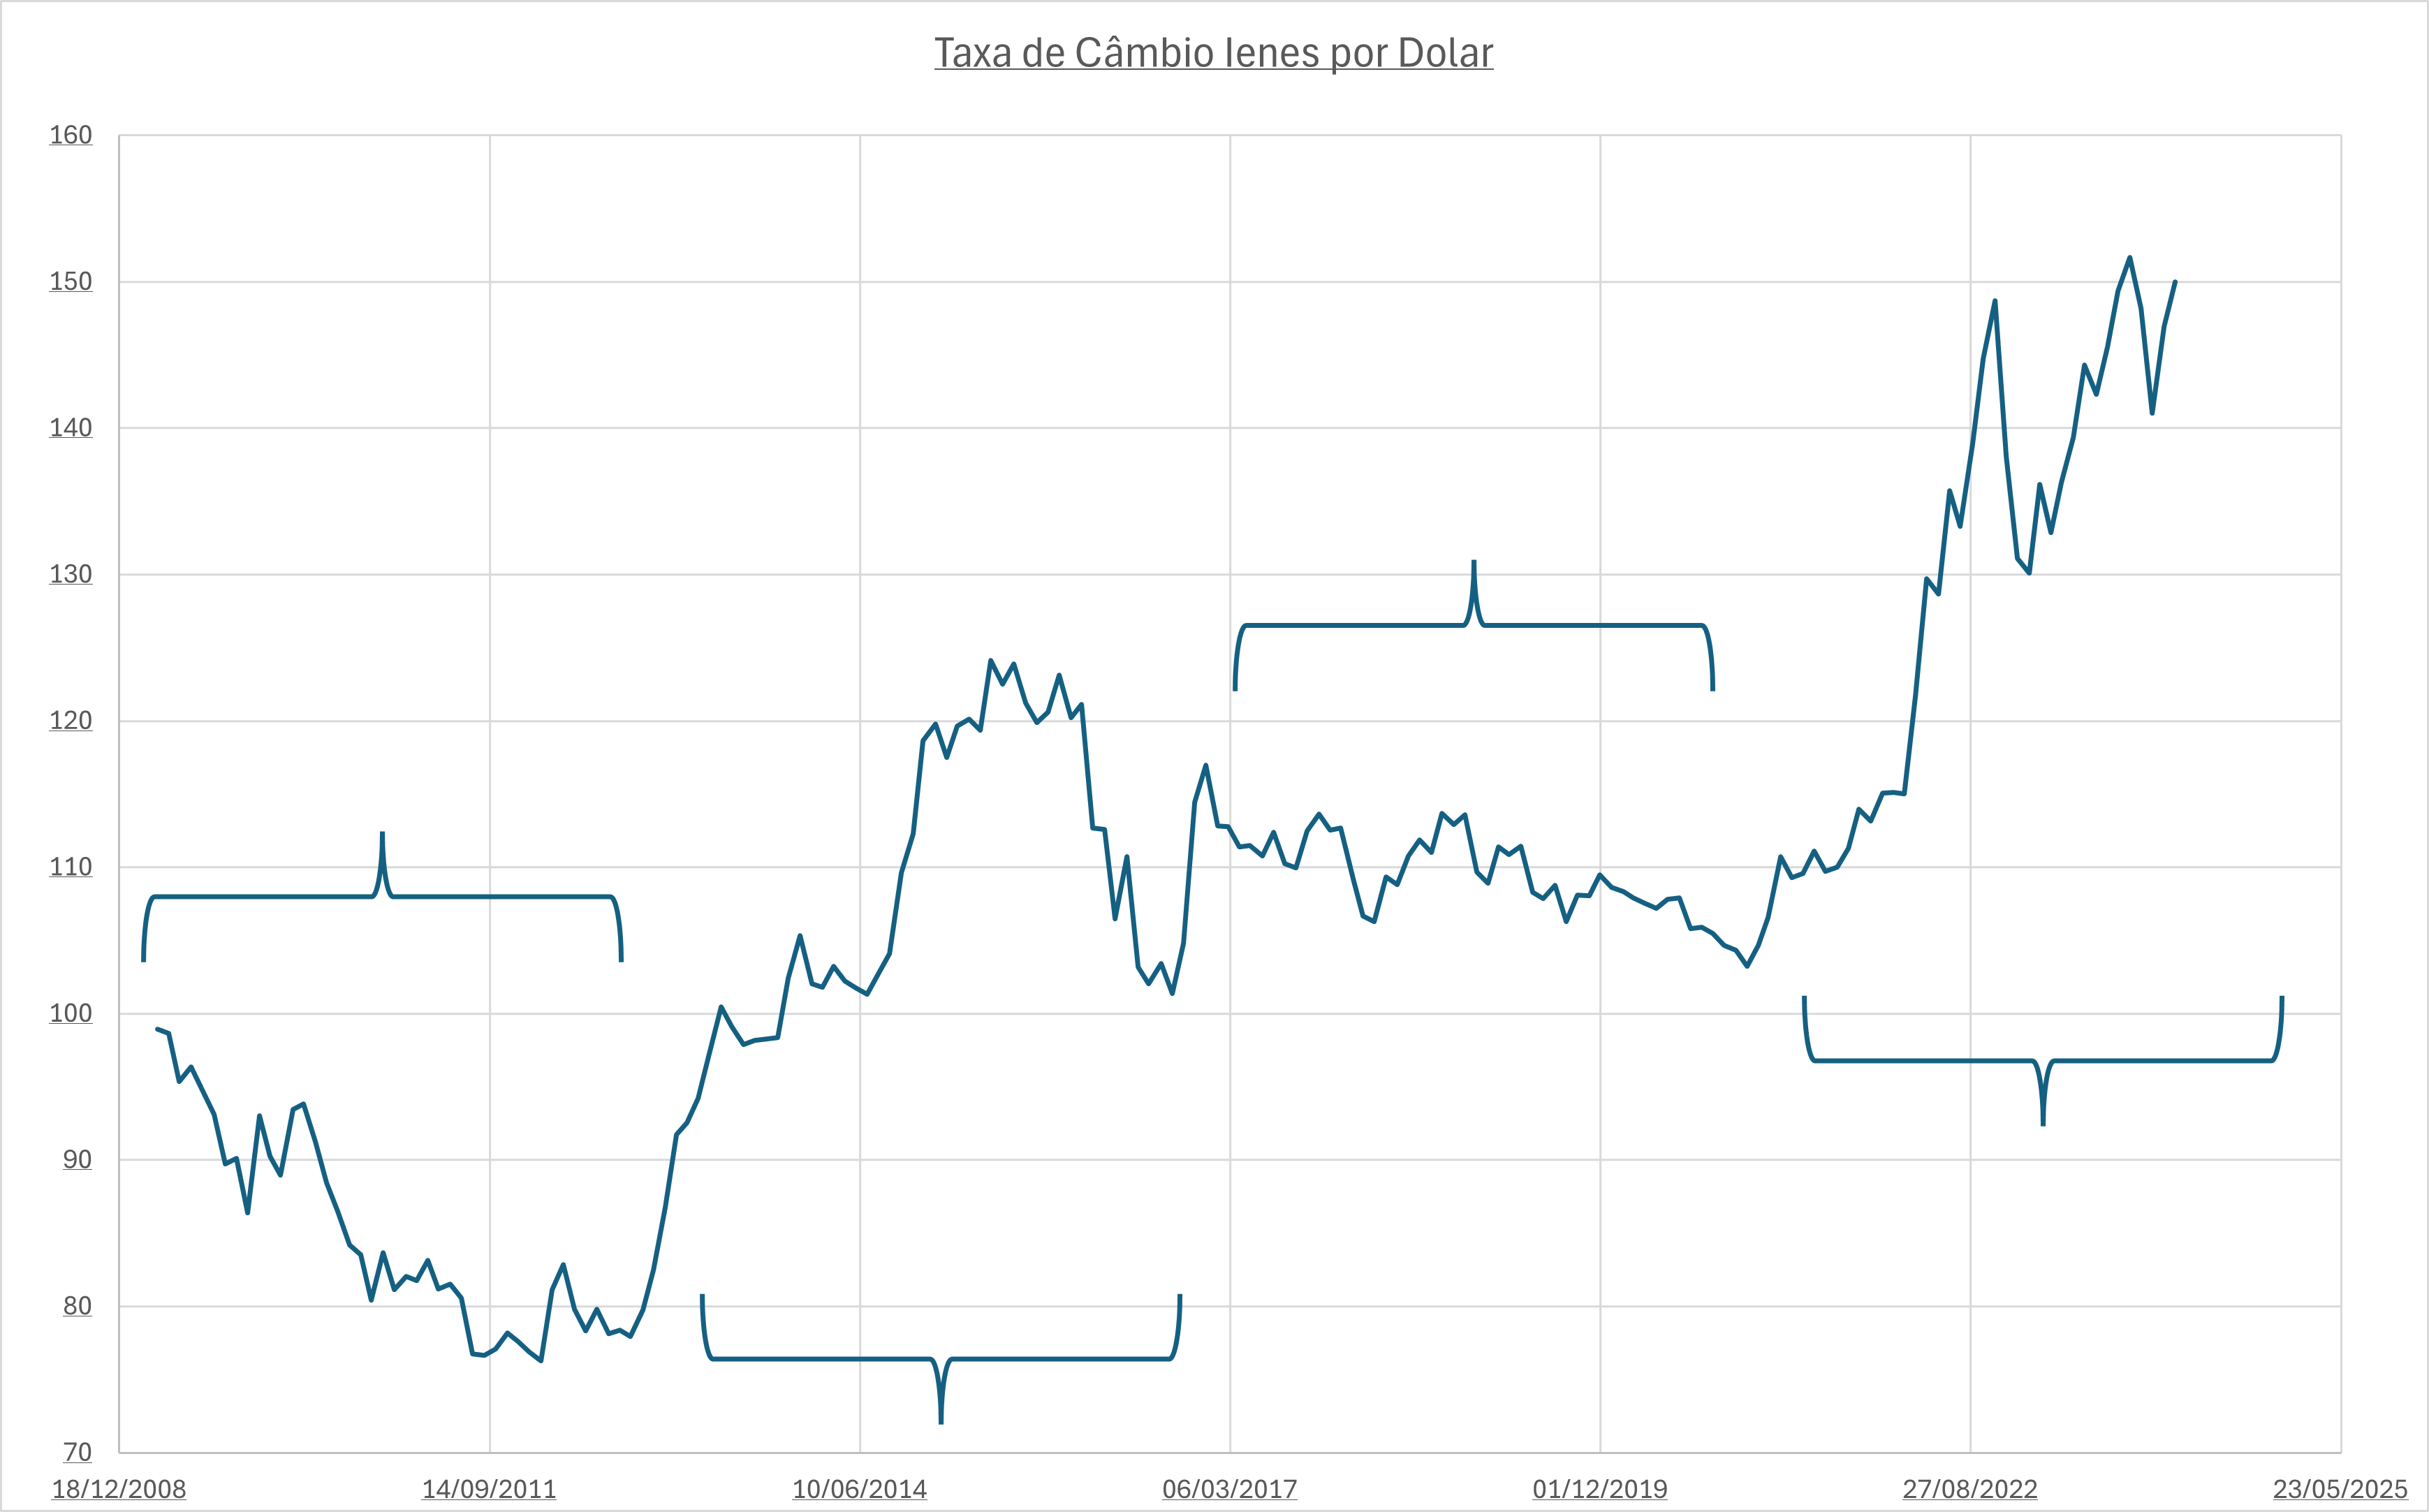
\includegraphics[width=0.75\textwidth]{Câmbio Iene Dolar.png}
    \label{fig:cambio}
    
    \footnotesize{Fonte: Elaborado pelos autores.}
    \end{figure}

Ao longo desses quatro períodos, podemos observar diferentes tendências na taxa de câmbio entre o iene e o dólar. No primeiro período, houve uma apreciação do iene em relação ao dólar, resultando em uma apreciação da taxa de câmbio. No segundo período, o dólar ganhou força em relação ao iene, revertendo a apreciação anterior e levando a uma depreciação da taxa de câmbio. No terceiro período, a taxa de câmbio entre as duas moedas mostrou uma certa estabilidade, sem grandes flutuações. No entanto, no último período, o dólar se fortaleceu significativamente em relação ao iene, resultando em uma maior depreciação da taxa de câmbio.

\subsection{\textbf{Análise de Variável Por Período}}
Antes de começarmos a análise, vamos definir os períodos que vamos trabalhar ; 1º período sera de março de 2009 até setembro de 2012, o 2º período será de setembro de 2012 até janeiro de 2016, o 3º período será   de janeiro de 2016 até dezembro de 2020 e o 4º período será de dezembro de 2020 até fevereiro de 2024.

    
\section{\textbf{Questão 2}}
A taxa de câmbio pode ser afetada por diversos fatores, como pelo produto (PIB), oferta monetária doméstica ou externa e taxa de juros nacional. Cada um desses fatores afeta a taxa de câmbio de diferentes formas.

Isso faz com que seja inviável comparar mais de um fator afetando a taxa de câmbio ao mesmo tempo. Para podermos entender melhor qual fator está contribuindo para a flutuação do câmbio, vamos analisar diferentes fatores e identificar aquele que melhor explica a taxa de câmbio.  

Sabendo disso podemos começar a análise das tendências das variáveis em cada período.

\subsubsection{\textbf{Oferta Monetária}}

No 1º período a oferta monetária no Japão se manteve relativamente constante, sofrendo oscilações que se compensam ao longo do tempo. Já no Estados Unidos ela sofreu uma perda significativa mas foi se recuperando.

No 2º período a oferta monetária no Japão atingiu novas máximas, mas repetiu o padrão do período anterior, sofreu oscilações que se compensavam ao longo do tempo. Já nos Estados Unidos, apesar de se recuperar da queda anterior, esse período foi marcado por um decrescimento da oferta monetária. 

No 3º período a oferta monetária do Japão começou a cair e isso só parou no final do período quando começou a subir drasticamente. Já a oferta monetária dos Estados Unidos continuou a sua tendência de queda, mas assim como no Japão, no final do período a oferta monetária subiu drasticamente.

No 4º período a oferta monetária do Japão teve uma crescimento enorme, algo jamais antes visto, mas logo depois se encerrou e começou a haver cortes severos, voltando para os padrões históricos anteriores. Já em relação a oferta monetária dos Estados Unidos, ela seguiu o mesmo do Japão, e logo após a máxima histórica, começou os corte, porém superiores a do Japão, atingindo uma míníma histórica pouco antes do final do período

\subsubsection{\textbf{Taxa de Juros}}
No 1º período ambas as taxa de juros eram relativamente constantes e baixas, a do Japão era realmente constante e a do Estados Unidos oscilava pouco e em torno de um valor baixo.

No 2º período , mais especificamente na metade do período , o Japão teve um corte de juros, marcando o início de uma taxa de juros negativa. Já os Estados Unidos , também começou a aumentar o juros na segunda metade do período.

No 3º período o Japão ainda continua com a taxa de juros negativa. Já os Estados Unidos atingiram um patamar alta da taxa de juros, mas que foi sucedido por cortes significativos logos após, voltando a padrões históricos.

No 4º período o Japão ainda continua com a taxa de juros negativa. Já os Estados Unidos , até chegar na metade deste período, ela se manteve baixa, após a metade a taxa de juros começou a sofrer aumentos cada vez mais sucessivos, atingindo uma máxima histórica.

\subsubsection{\textbf{Inflação}}
No 1º período a inflação do Japão teve uma queda abrupta, mas que aos poucos voltou a subir e se manter estável. Já a inflação dos Estados Unidos teve um aumento significativo, mas se mantendo estável logo após.

No 2º período, a inflação do Japão teve um crescimento abrupto em pouco tempo, mas após atingir a máxima, começou a cair, voltando para padrões anteriores. Já a inflação dos Estados Unidos se manteve relativamente constante, oscilando em torno de uma média.

No 3º período a inflação do Japão se manteve estável ao padrão anterior, oscilando em torno de uma média, mas com uma tendência de queda. Já a inflação do Estados Unidos também se manteve em torno de uma média, oscilando.

No 4º período a inflação do Japão teve um início de queda, mas que foi logo sucedido por uma disparada, que após atingir a máxima, começou a sofrer quedas. Já a inflação do Estados Unidos, seguiu o mesmo padrão do Japão, começou com uma queda, sucedida com um alto crescimento, mas depois da máxima, foi caindo paulatinamente. 

\subsubsection{\textbf{PIB}}
No 1º período, o PIB do Japão começou decrescendo muito mas logo cresceu a um ponto eu que haviam variações menores entre crescimento e decrescimento. Já o EUA, tiveram uma experiencia parecida mas com oscilações menores.

No 2º período, o Japão começou no mesmo ritmo que tinha no período anterior até 2015, quando começaram a ter um crescimento mais frequente. Já os Estados Unidos, mantiveram o passo do período passado.

No 3º período, o Japão com crescimentos um pouco menores do que os Estados Unidos teve uma grande baixa em 2020. A baixa dos Estados Unidos foi semelhante.

No 4º período, os dois países tiveram grandes altas na metade de 2021 mas voltaram a padrões de crescimento baixo logo após

\subsection{\textbf{Relação do Câmbio com a Oferta Monetária}}

A princípio, a oferta monetária doméstica de moeda (Ms) tem efeito sobre a taxa de câmbio (E). Quando a quantidade de moedas na economia aumenta, a relação pura entre essa e a moeda estrangeira muda de modo que uma maior quantidade de moeda doméstica deverá ser utilizada para comprar a outra (Iene/Dólar). 

Consequentemente, nessa mesma relação, o valor relativo da moeda estrangeira aumenta, isso pode ser visto na Figura~\ref{fig:cambioOfertaJapão}.

 \begin{figure}[H]
    \centering
    \caption{Gráfico da Taxa de Câmbio Iene por Dólar e Oferta Monetária do Japão} 
    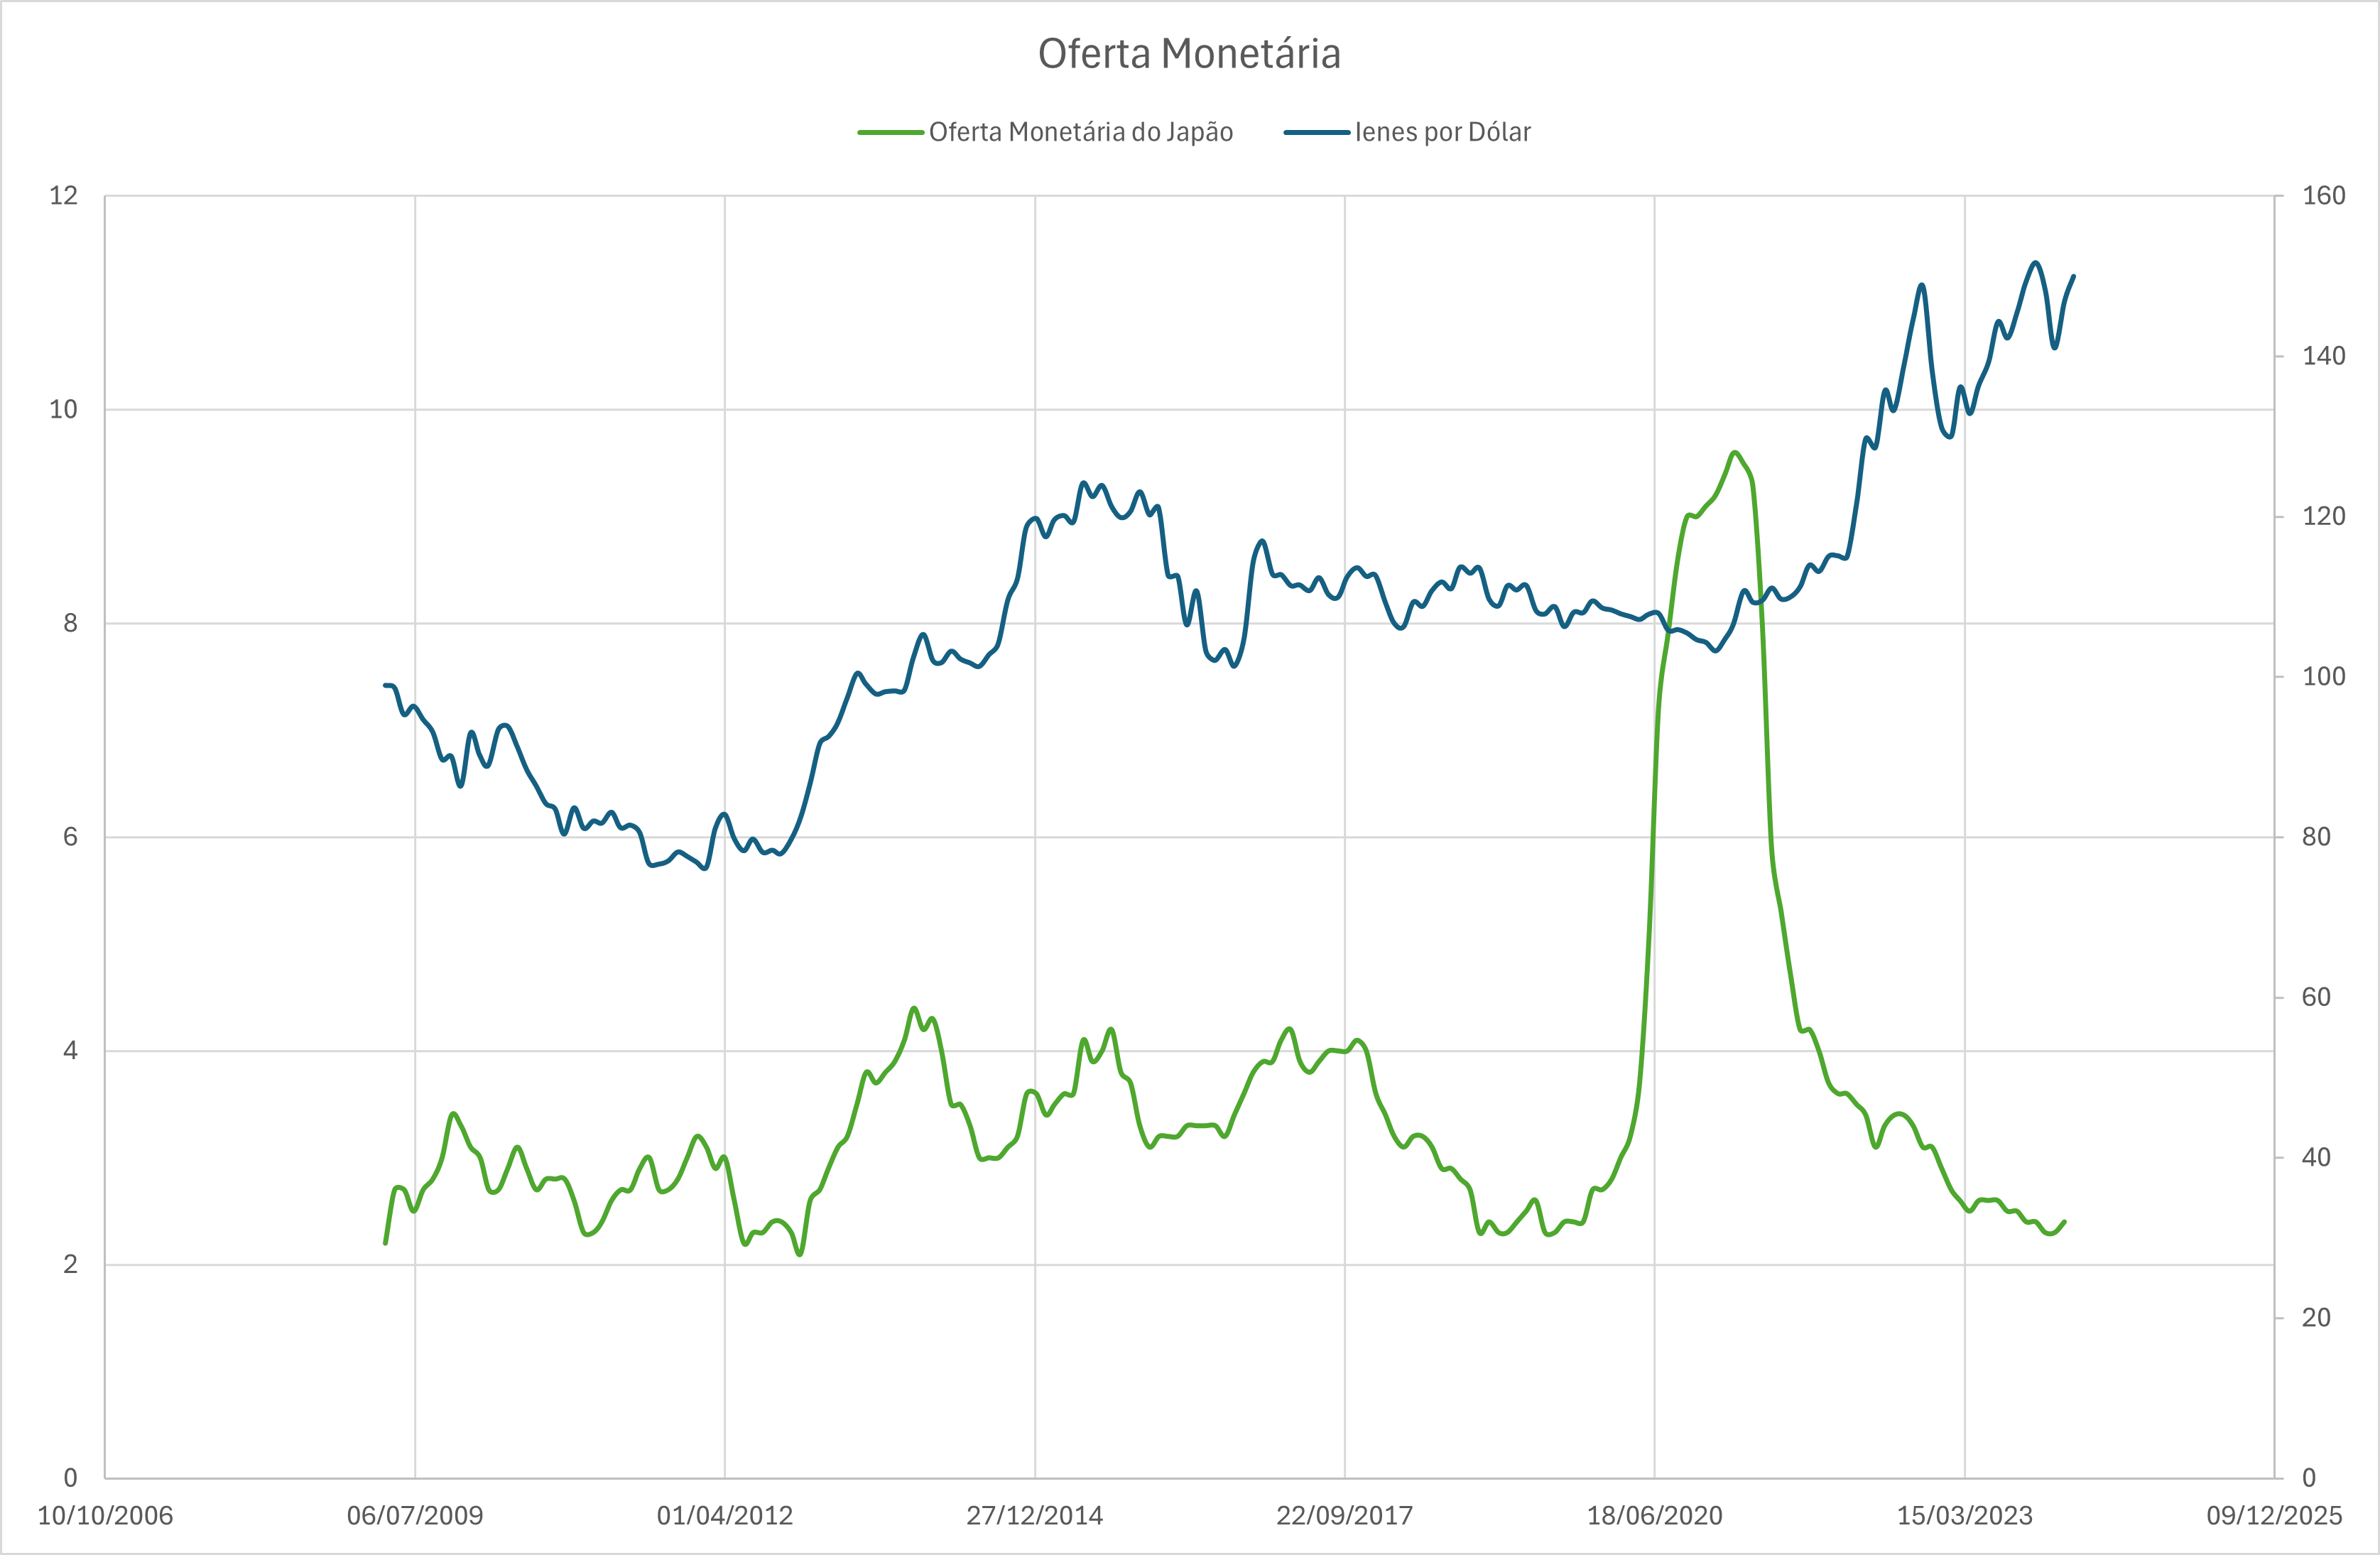
\includegraphics[width=0.75\textwidth]{Oferta monetária Japão.png}
    \label{fig:cambioOfertaJapão}
    
    \footnotesize{Fonte: Elaborado pelos autores.}
    \end{figure}

No final de 2019, após anos se comportando da mesma maneira, a oferta de moedas no Japão se elevou até seu pico em 2020, o que deveria ter desvalorizado seu câmbio, porém, como analisado anteriormente, o câmbio é uma medida relativa.
Ao observar a Figura~\ref{fig:cambioOfertaEUA} a seguir, é possível identificar depreciação do dólar no mesmo período.

 \begin{figure}[H]
    \centering
    \caption{Gráfico da Taxa de Câmbio Iene por Dólar e Oferta Monetária do EUA} 
    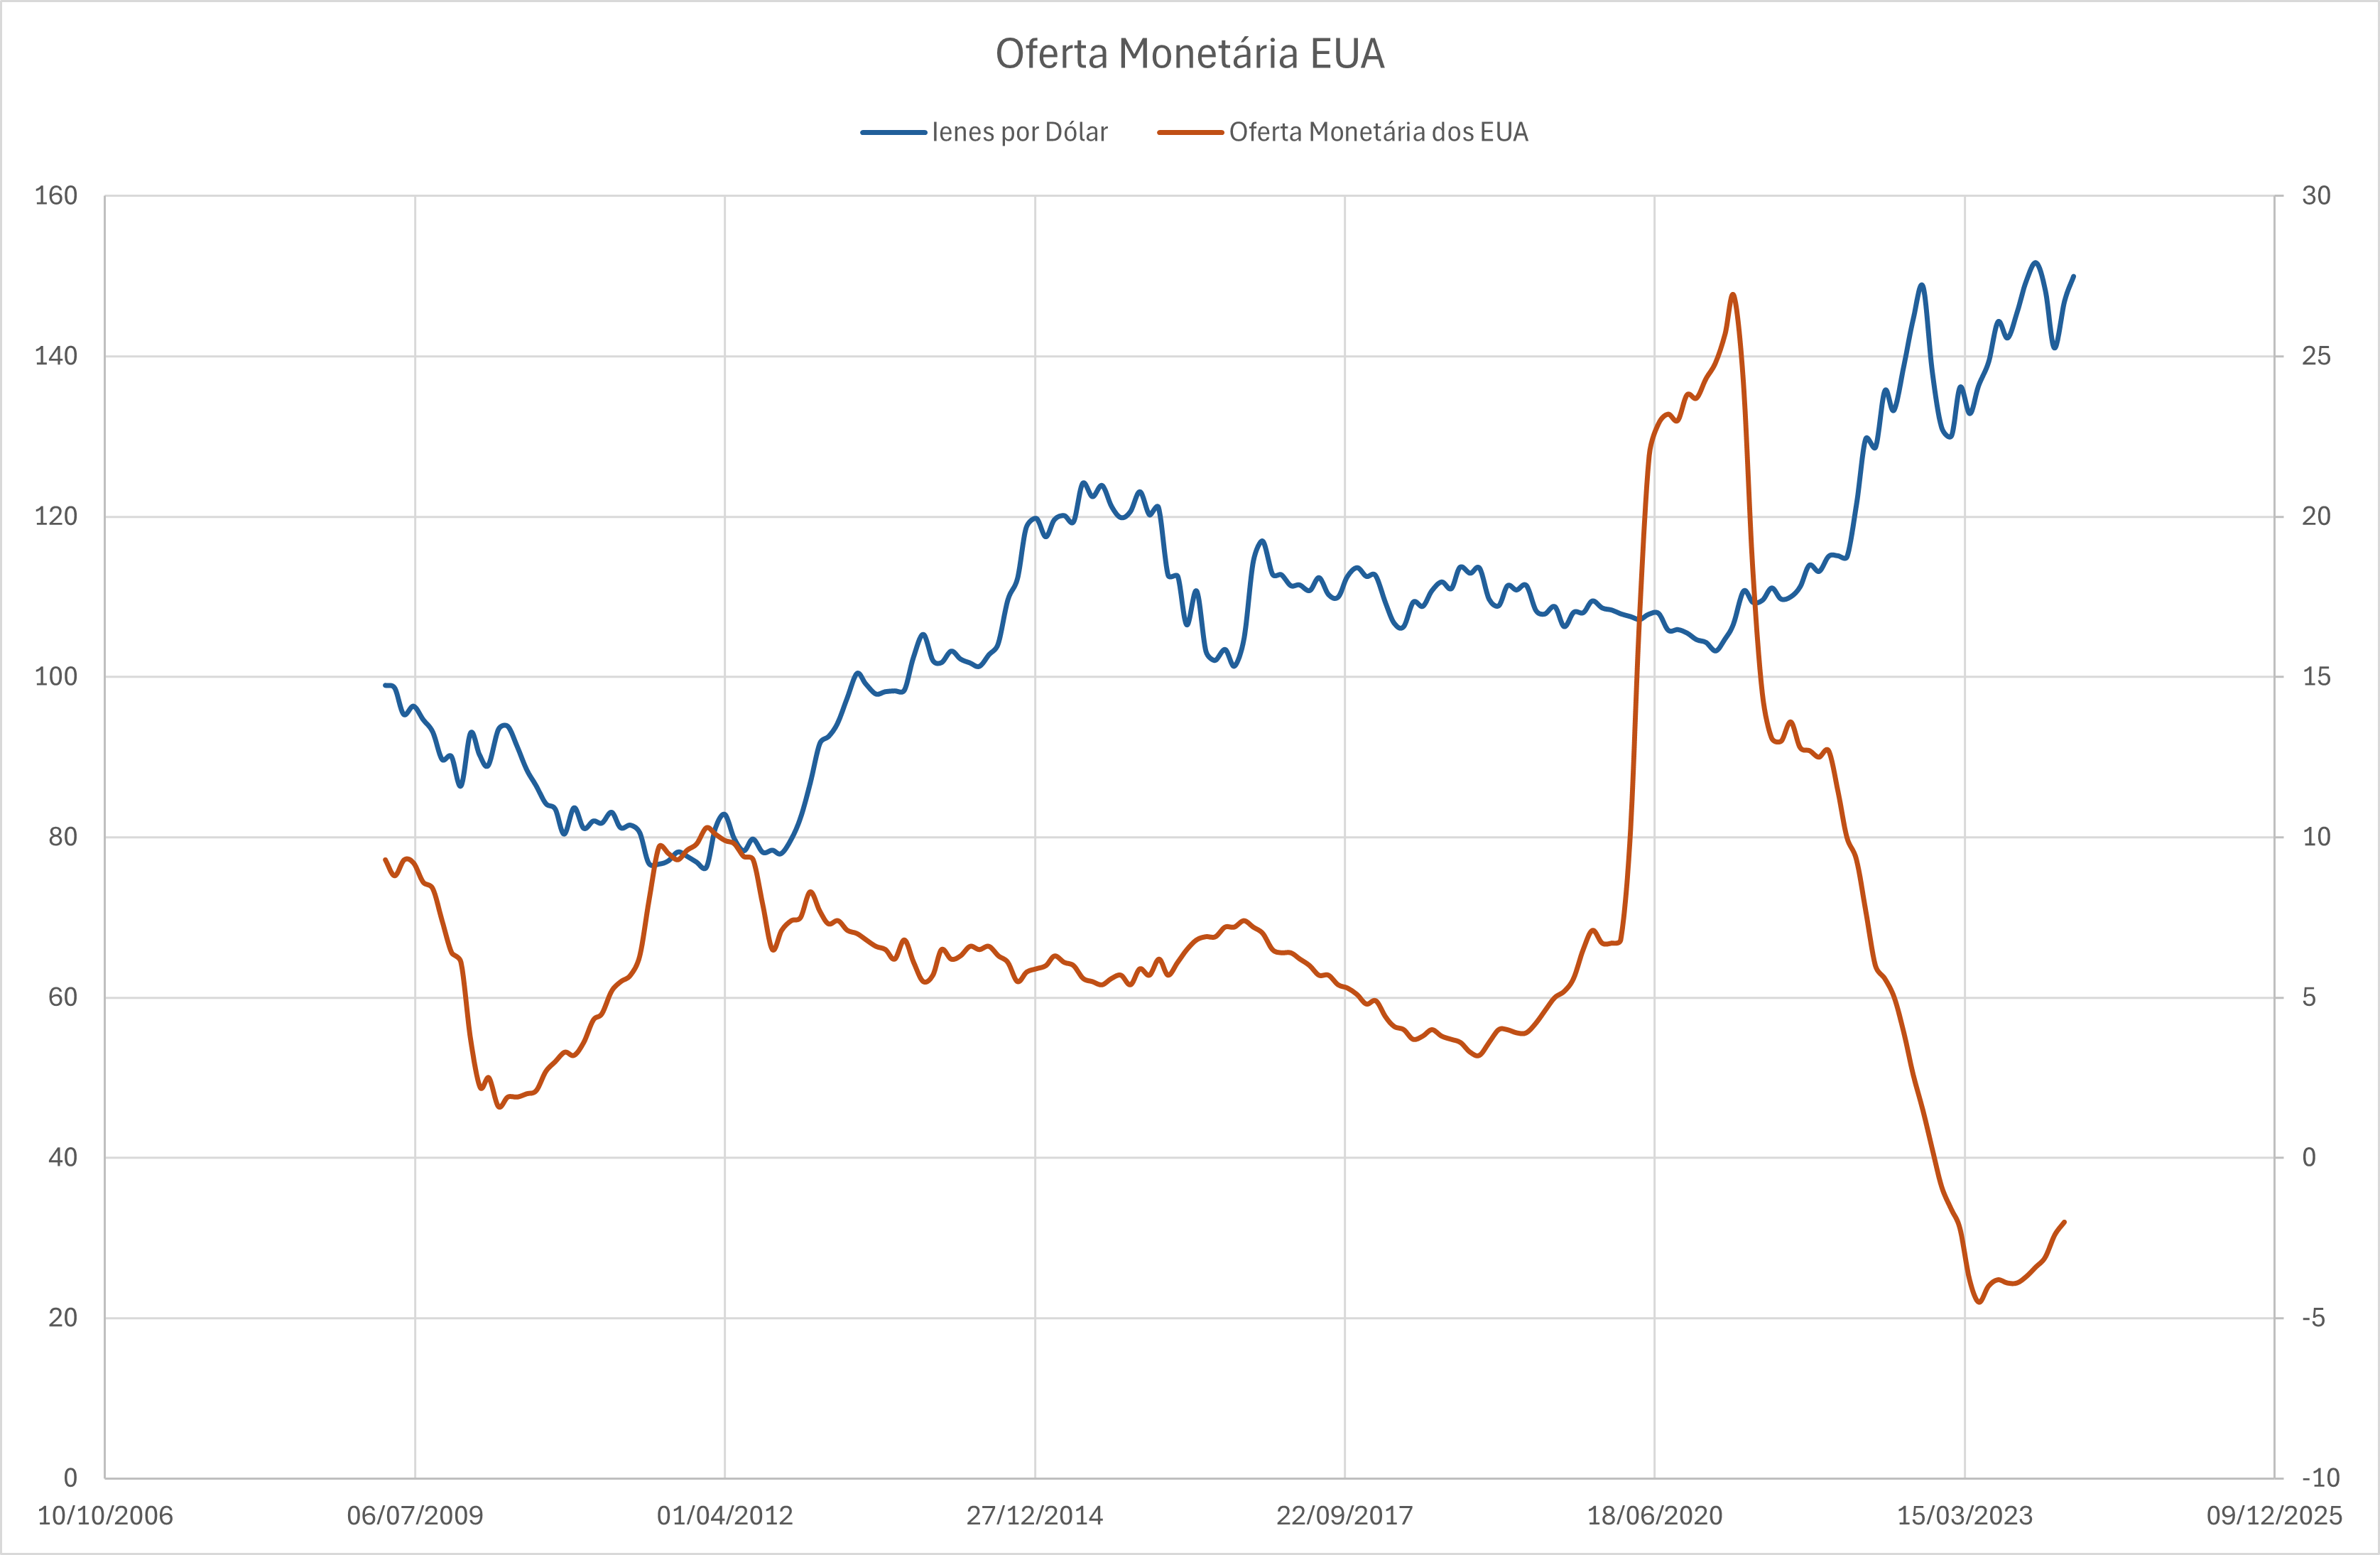
\includegraphics[width=0.75\textwidth]{Oferta de Moeda EUA.png}
    \label{fig:cambioOfertaEUA}
    
    \footnotesize{Fonte: Elaborado pelos autores.}
    \end{figure}

\subsection{\textbf{Relação do Câmbio com as Taxas de Juros}}
A intuição econômica geral indica que a taxa de juros interna (R) tem um papel significativo na determinação da taxa de câmbio (E). Quando R aumenta, a demanda pela moeda local tende a crescer, impulsionada pelo aumento na rentabilidade dos ativos denominados nessa moeda. Esse crescimento na demanda resulta em uma valorização da moeda local. Essa valorização, por sua vez, tem um efeito positivo em E, levando à sua apreciação. Analogamente, um excesso de oferta de moeda estrangeira provoca sua desvalorização, o que consequentemente leva à apreciação de E.

A relação entre o câmbio ienes por dólar (E) com a taxa de juros japonesa pode ser vista na Figura~\ref{fig:cambioJurosJapao}
 \begin{figure}[H]
    \centering
    \caption{Gráfico da Taxa de Câmbio Iene por Dólar e Taxa de Juros do Japão} 
    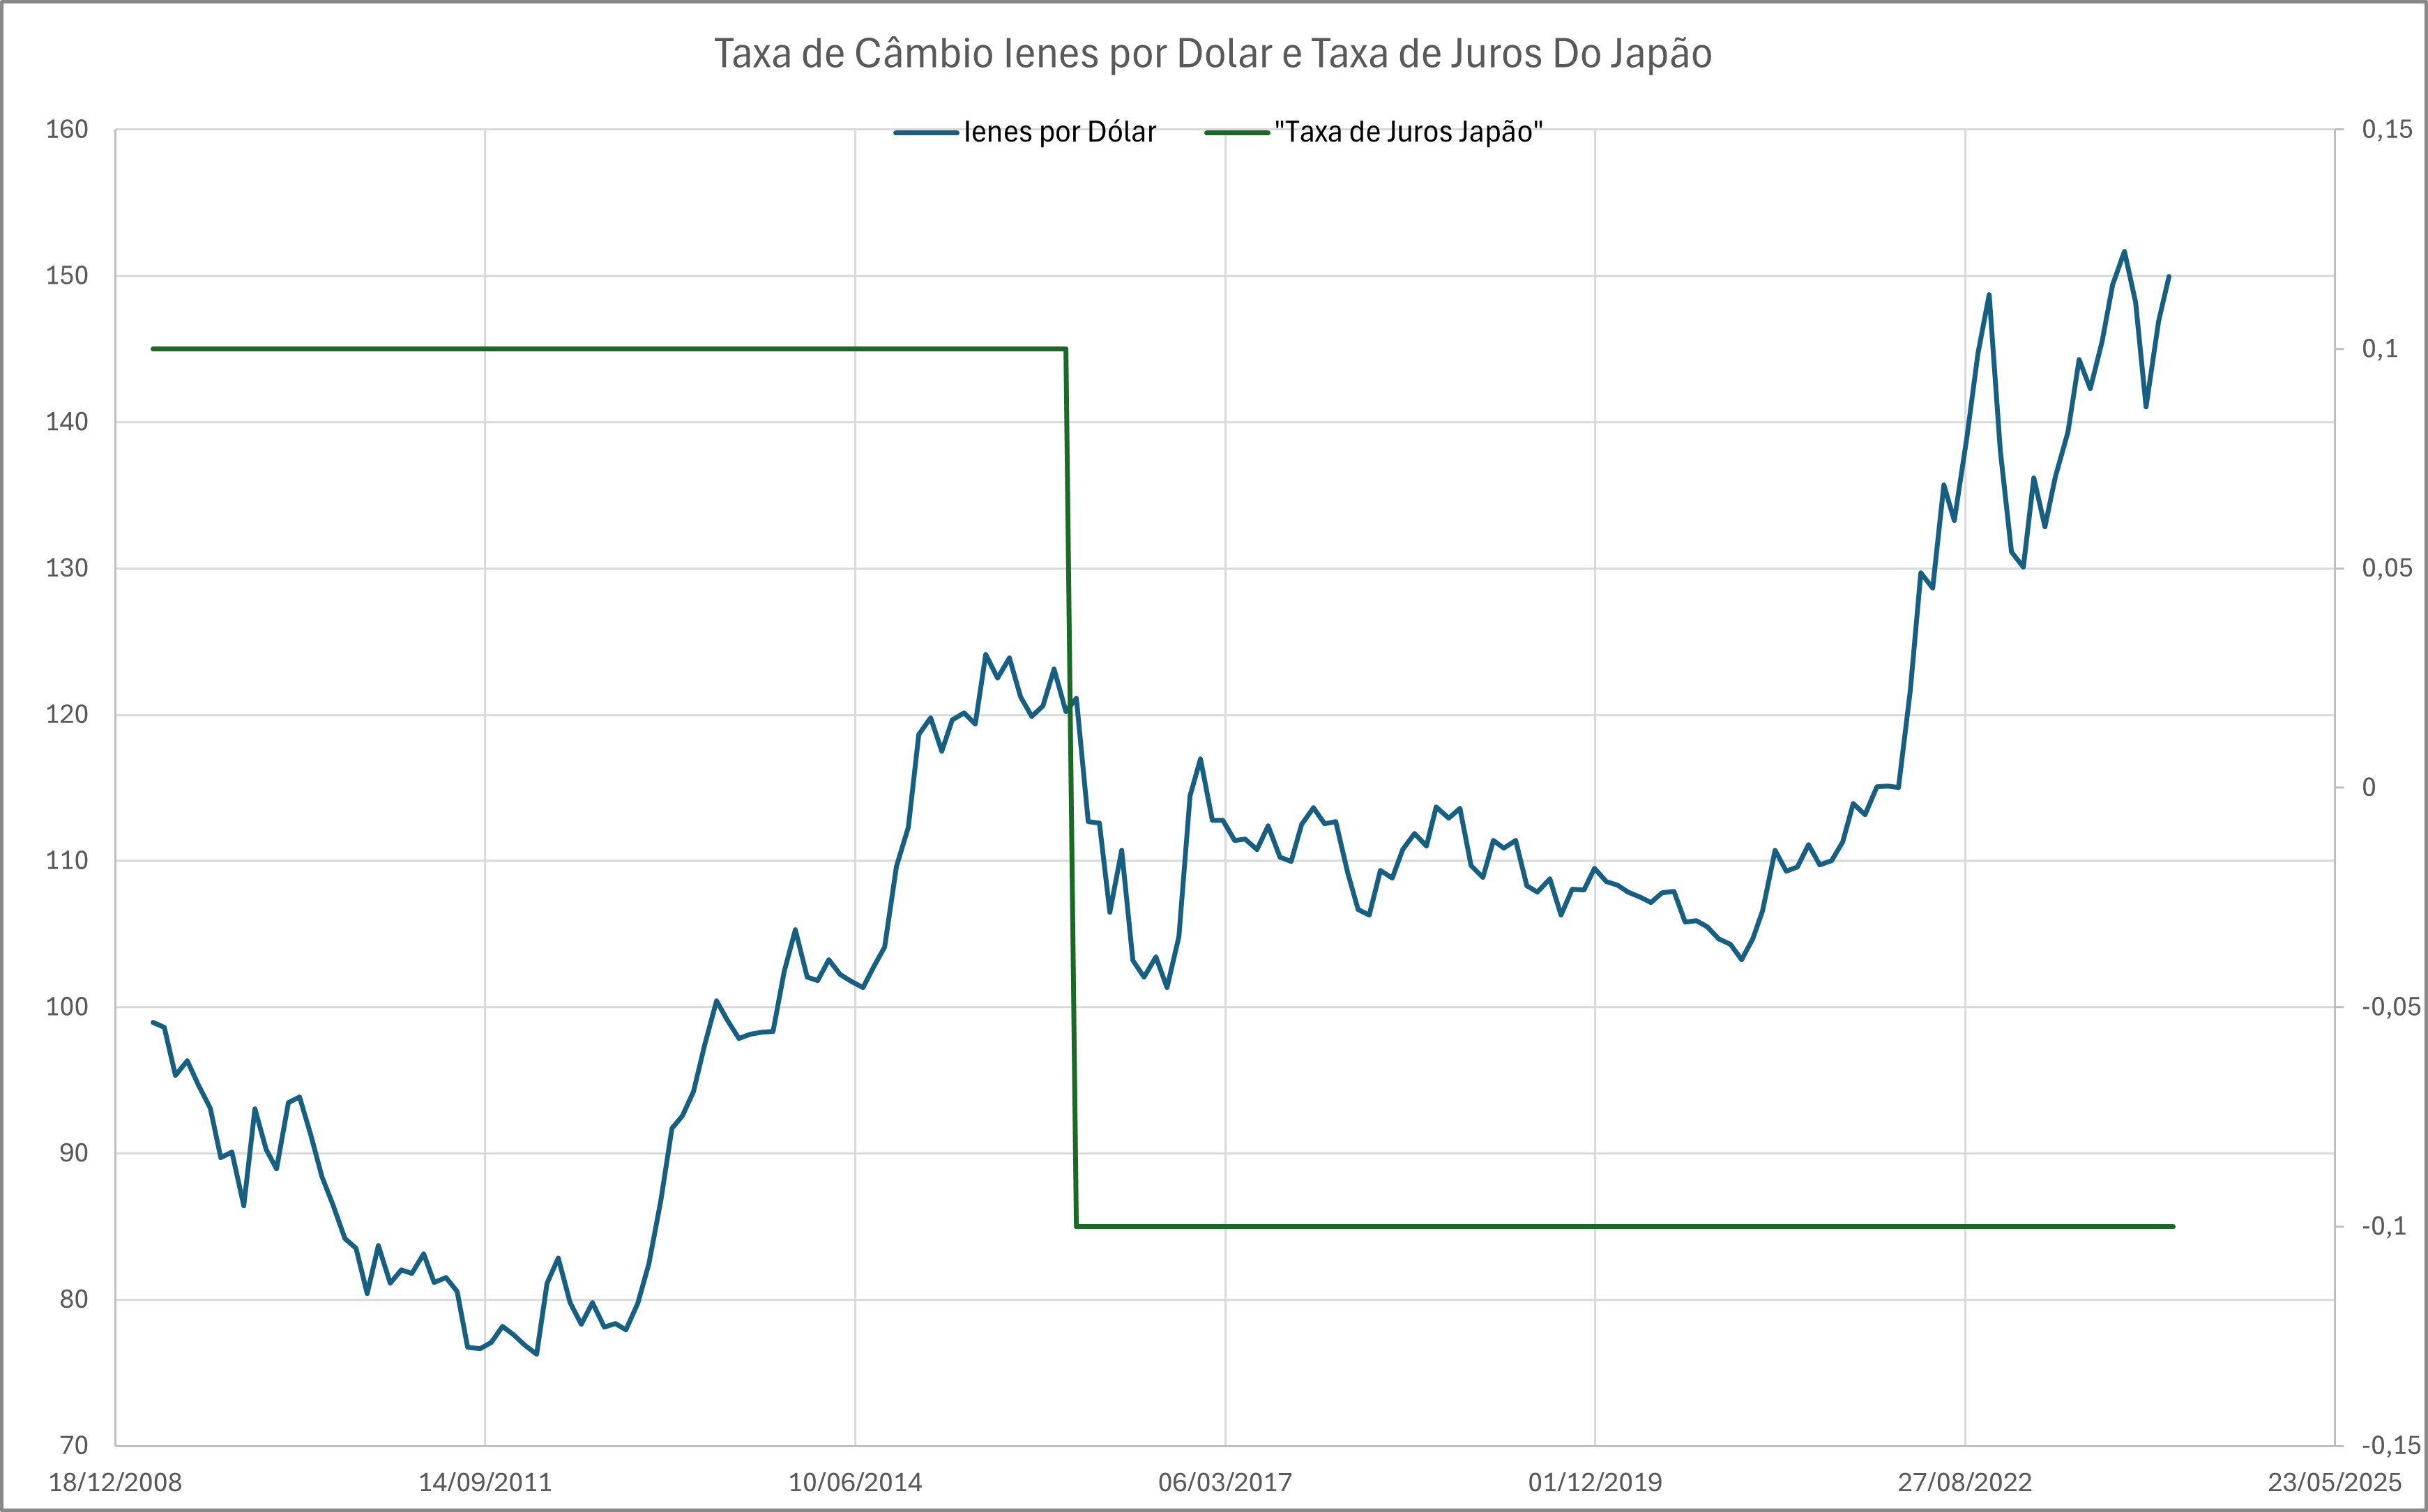
\includegraphics[width=0.75\textwidth]{Câmbio e Juros japoneses.png}
    \label{fig:cambioJurosJapao}
    
    \footnotesize{Fonte: Elaborado pelos autores.}
    \end{figure}

Durante um longo período, o Japão manteve uma taxa de juros de 0,1\%, considerada muito baixa. Isso incentivava a desvalorização do iene em relação ao dólar, resultando na depreciação cambial, ou seja, era preciso mais ienes para adquirir um dólar. No entanto, em 29 de fevereiro de 2016, houve uma redução na já baixa taxa de juros, estabelecendo a nova taxa básica de juros japonesa em -0,1\%. Isso implica que investir em títulos públicos seria equivalente a uma perda de poder de compra.

Esse fato intensificou ainda mais a demanda por dólares, reiterando o processo de depreciação da moeda e do câmbio interno.

A relação entre o câmbio ienes por dólar (E) com a taxa de juros estadunidense pode ser vista na  Figura~\ref{fig:cambioJurosEUA}.
 \begin{figure}[H]
    \centering
    \caption{Gráfico da Taxa de Câmbio Iene por Dólar e Taxa de Juros dos Estados Unidos} 
    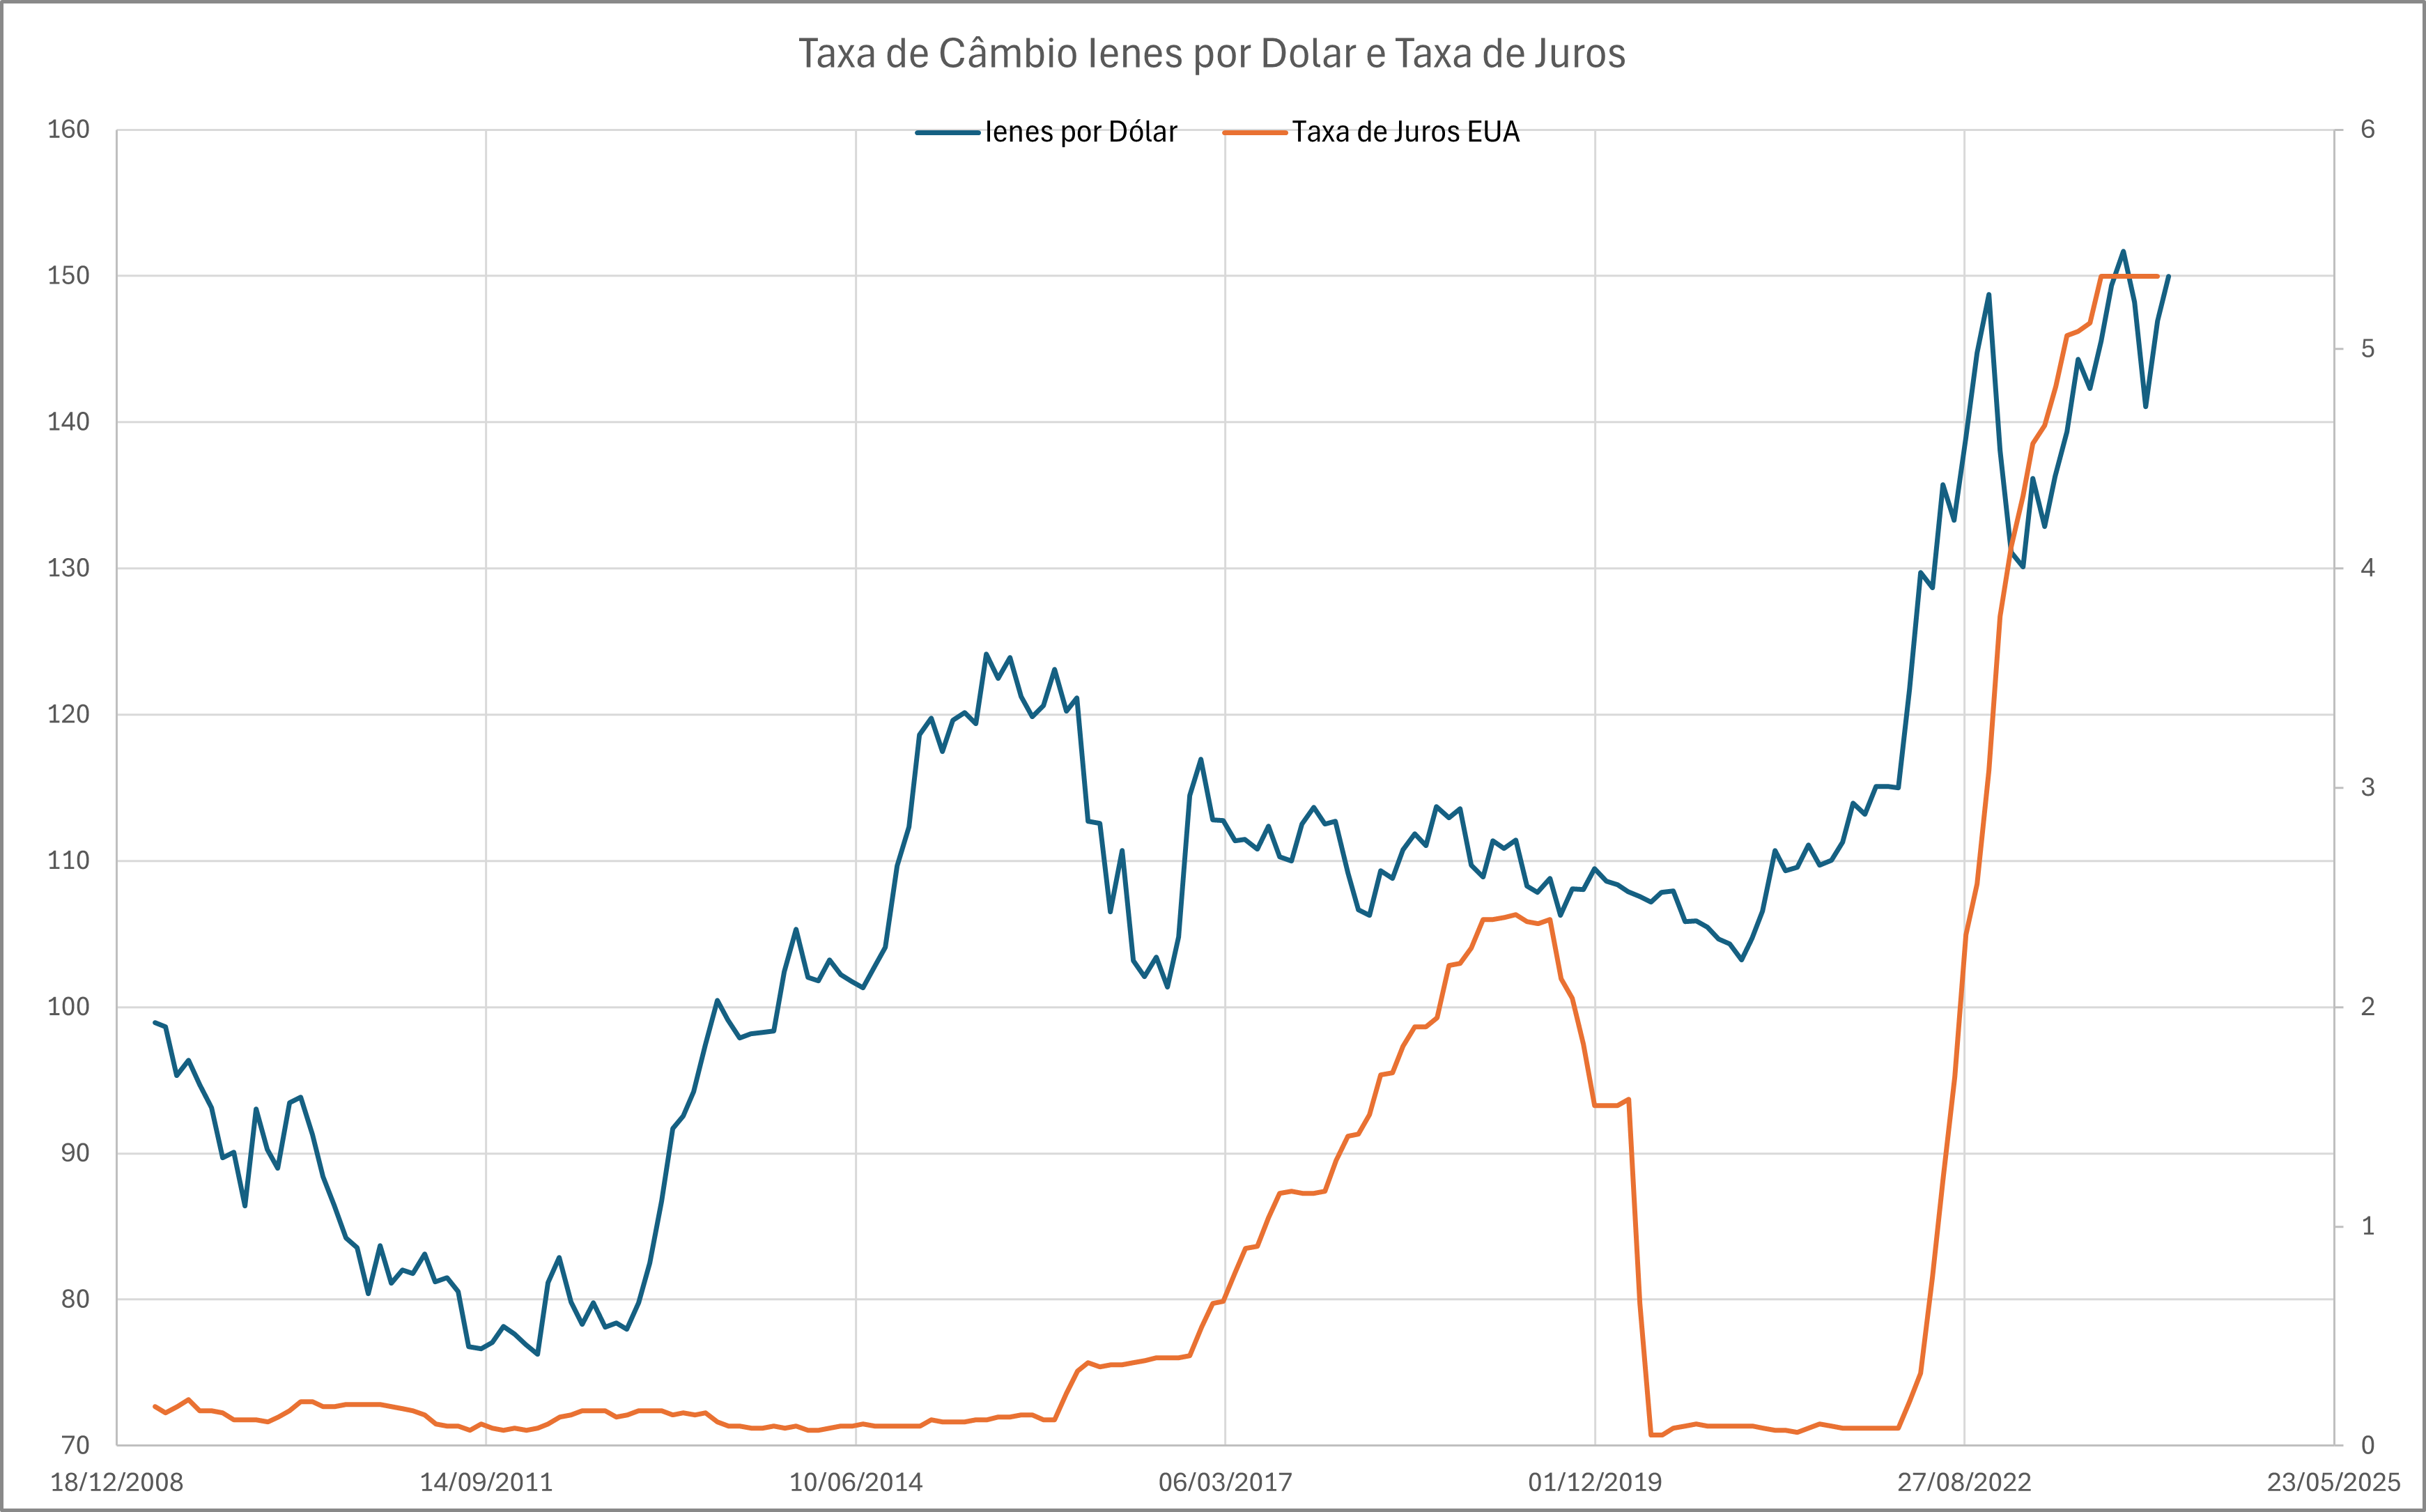
\includegraphics[width=0.75\textwidth]{Câmbio e Juros estadunidense.png}
    \label{fig:cambioJurosEUA}
    
    \footnotesize{Fonte: Elaborado pelos autores.}
    \end{figure}

Durante um longo período, a taxa de juros básica dos Estados Unidos permaneceu próxima de zero até 30 de agosto de 2015. Nessa data, houve um salto significativo, atingindo um pico de 2,4\% em 31 de julho de 2019. Isso marcou o início de um período de grandes cortes na taxa de juros, retornando aos níveis vistos antes de 2015.

A lógica econômica por trás desse aumento na taxa de juros seria um aumento na demanda por dólares, impulsionado por um aumento no retorno dos ativos denominados em dólares. Isso resulta em uma valorização do dólar, que por sua vez leva a uma depreciação cambial, dada a desvalorização do iene.

Em 28 de fevereiro de 2022, a taxa de juros dos Estados Unidos começou a subir de forma significativa, atingindo um recorde histórico de 5,33\% em 31 de agosto de 2023. O mesmo raciocínio econômico se aplica novamente: o dólar se valoriza, resultando em uma depreciação cambial, paralelamente à desvalorização do iene.

\subsection{\textbf{Relação do Câmbio com as Inflações}}

A lógica econômica geral sugere que a inflação interna tem um papel crucial na determinação da taxa de câmbio (E). Quando a inflação aumenta, o poder de compra da moeda local tende a diminuir. Isso leva a uma maior demanda por moeda estrangeira, resultando em uma desvalorização da moeda local. Essa desvalorização tem um impacto negativo em E, levando à sua depreciação. De maneira análoga, uma diminuição na inflação fortalece o poder de compra da moeda local, o que, por sua vez, resulta na apreciação de E.

No caso da relação entre o câmbio ienes por dólar (E) com a inflação japonesa, podemos ver na Figura~\ref{fig:cambioInflacaoJapao}.
 \begin{figure}[H]
    \centering
    \caption{Gráfico da Taxa de Câmbio Iene por Dólar e Inflação do Japão} 
    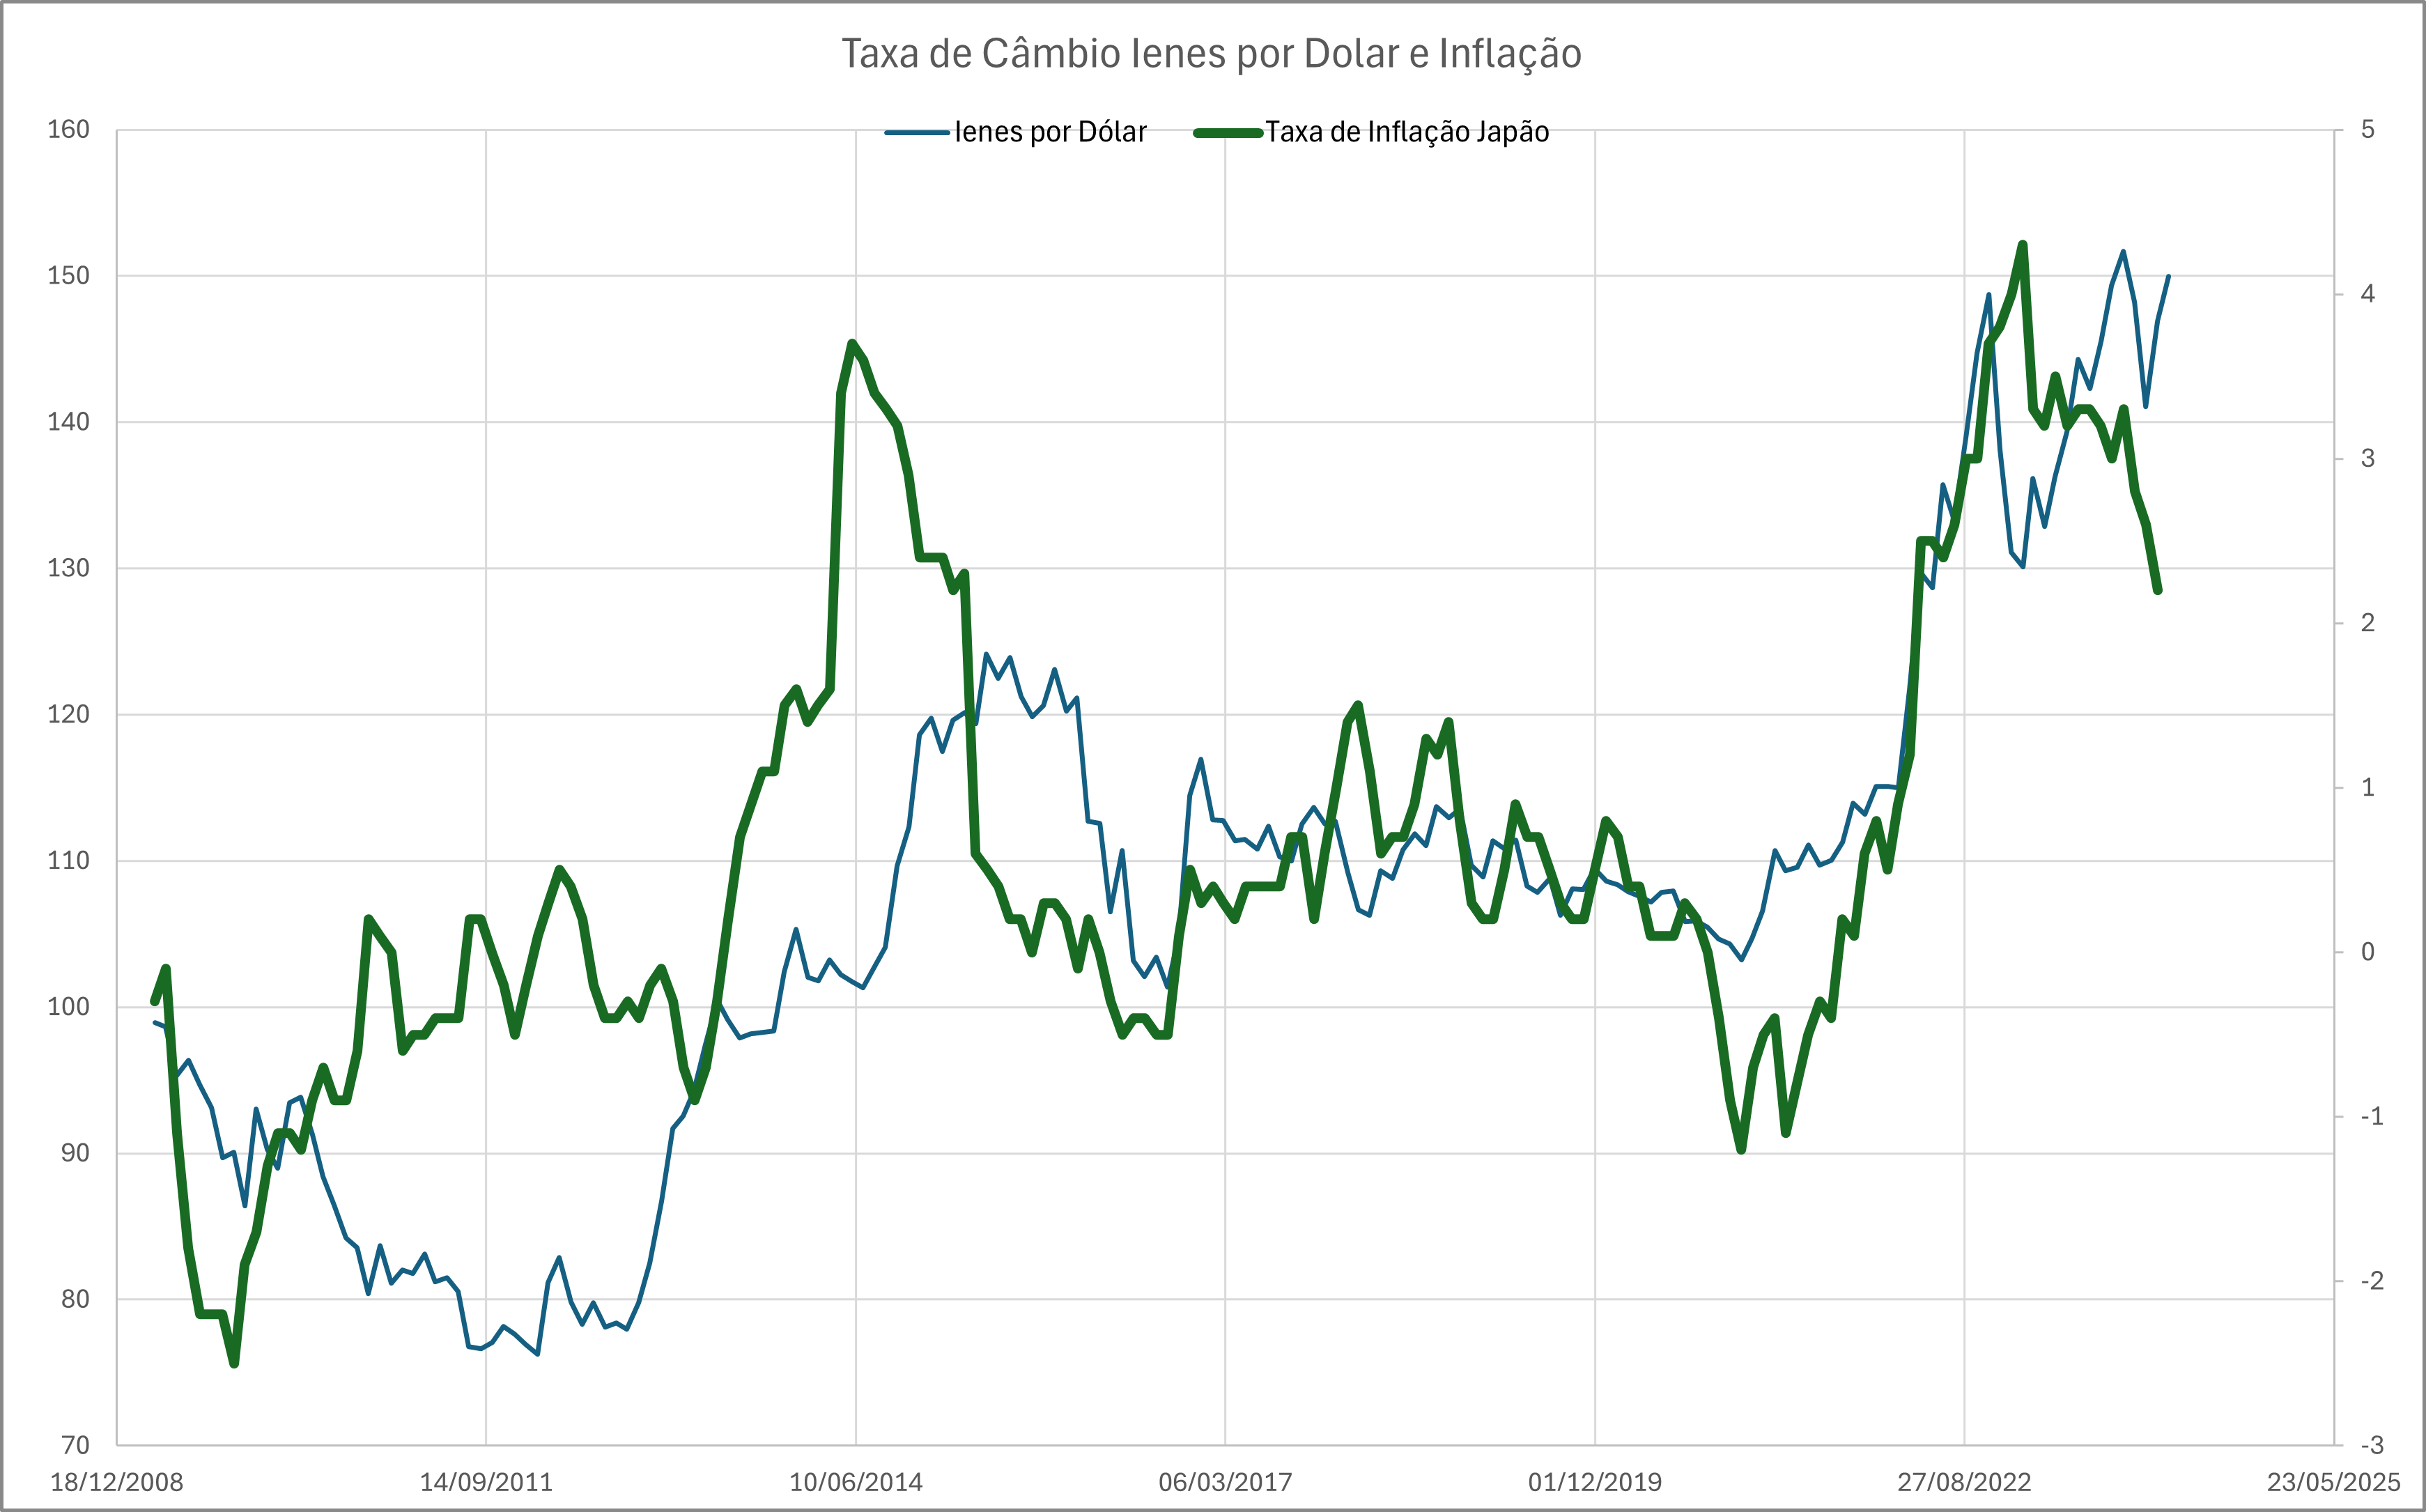
\includegraphics[width=0.75\textwidth]{Câmbio e Inflação japonesa.png}
    \label{fig:cambioInflacaoJapao}
    
    \footnotesize{Fonte: Elaborado pelos autores.}
    \end{figure}

Entre 31 de março de 2009 e 31 de março de 2013, o Japão experimentou um período de inflação interna crescente. Esse fenômeno resultou na desvalorização da moeda local. Intuitivamente, a desvalorização do iene leva a uma desvalorização cambial, refletida no fortalecimento do dólar, que é impulsionado pelo aumento da demanda pela moeda estrangeira. 

No caso da relação entre o câmbio ienes por dólar (E) com a inflação estadunidense, podemos ver na Figura~\ref{fig:cambioInflacaoEUA}.
 \begin{figure}[H]
    \centering
    \caption{Gráfico da Taxa de Câmbio Iene por Dólar e Inflação dos Estados Unidos} 
    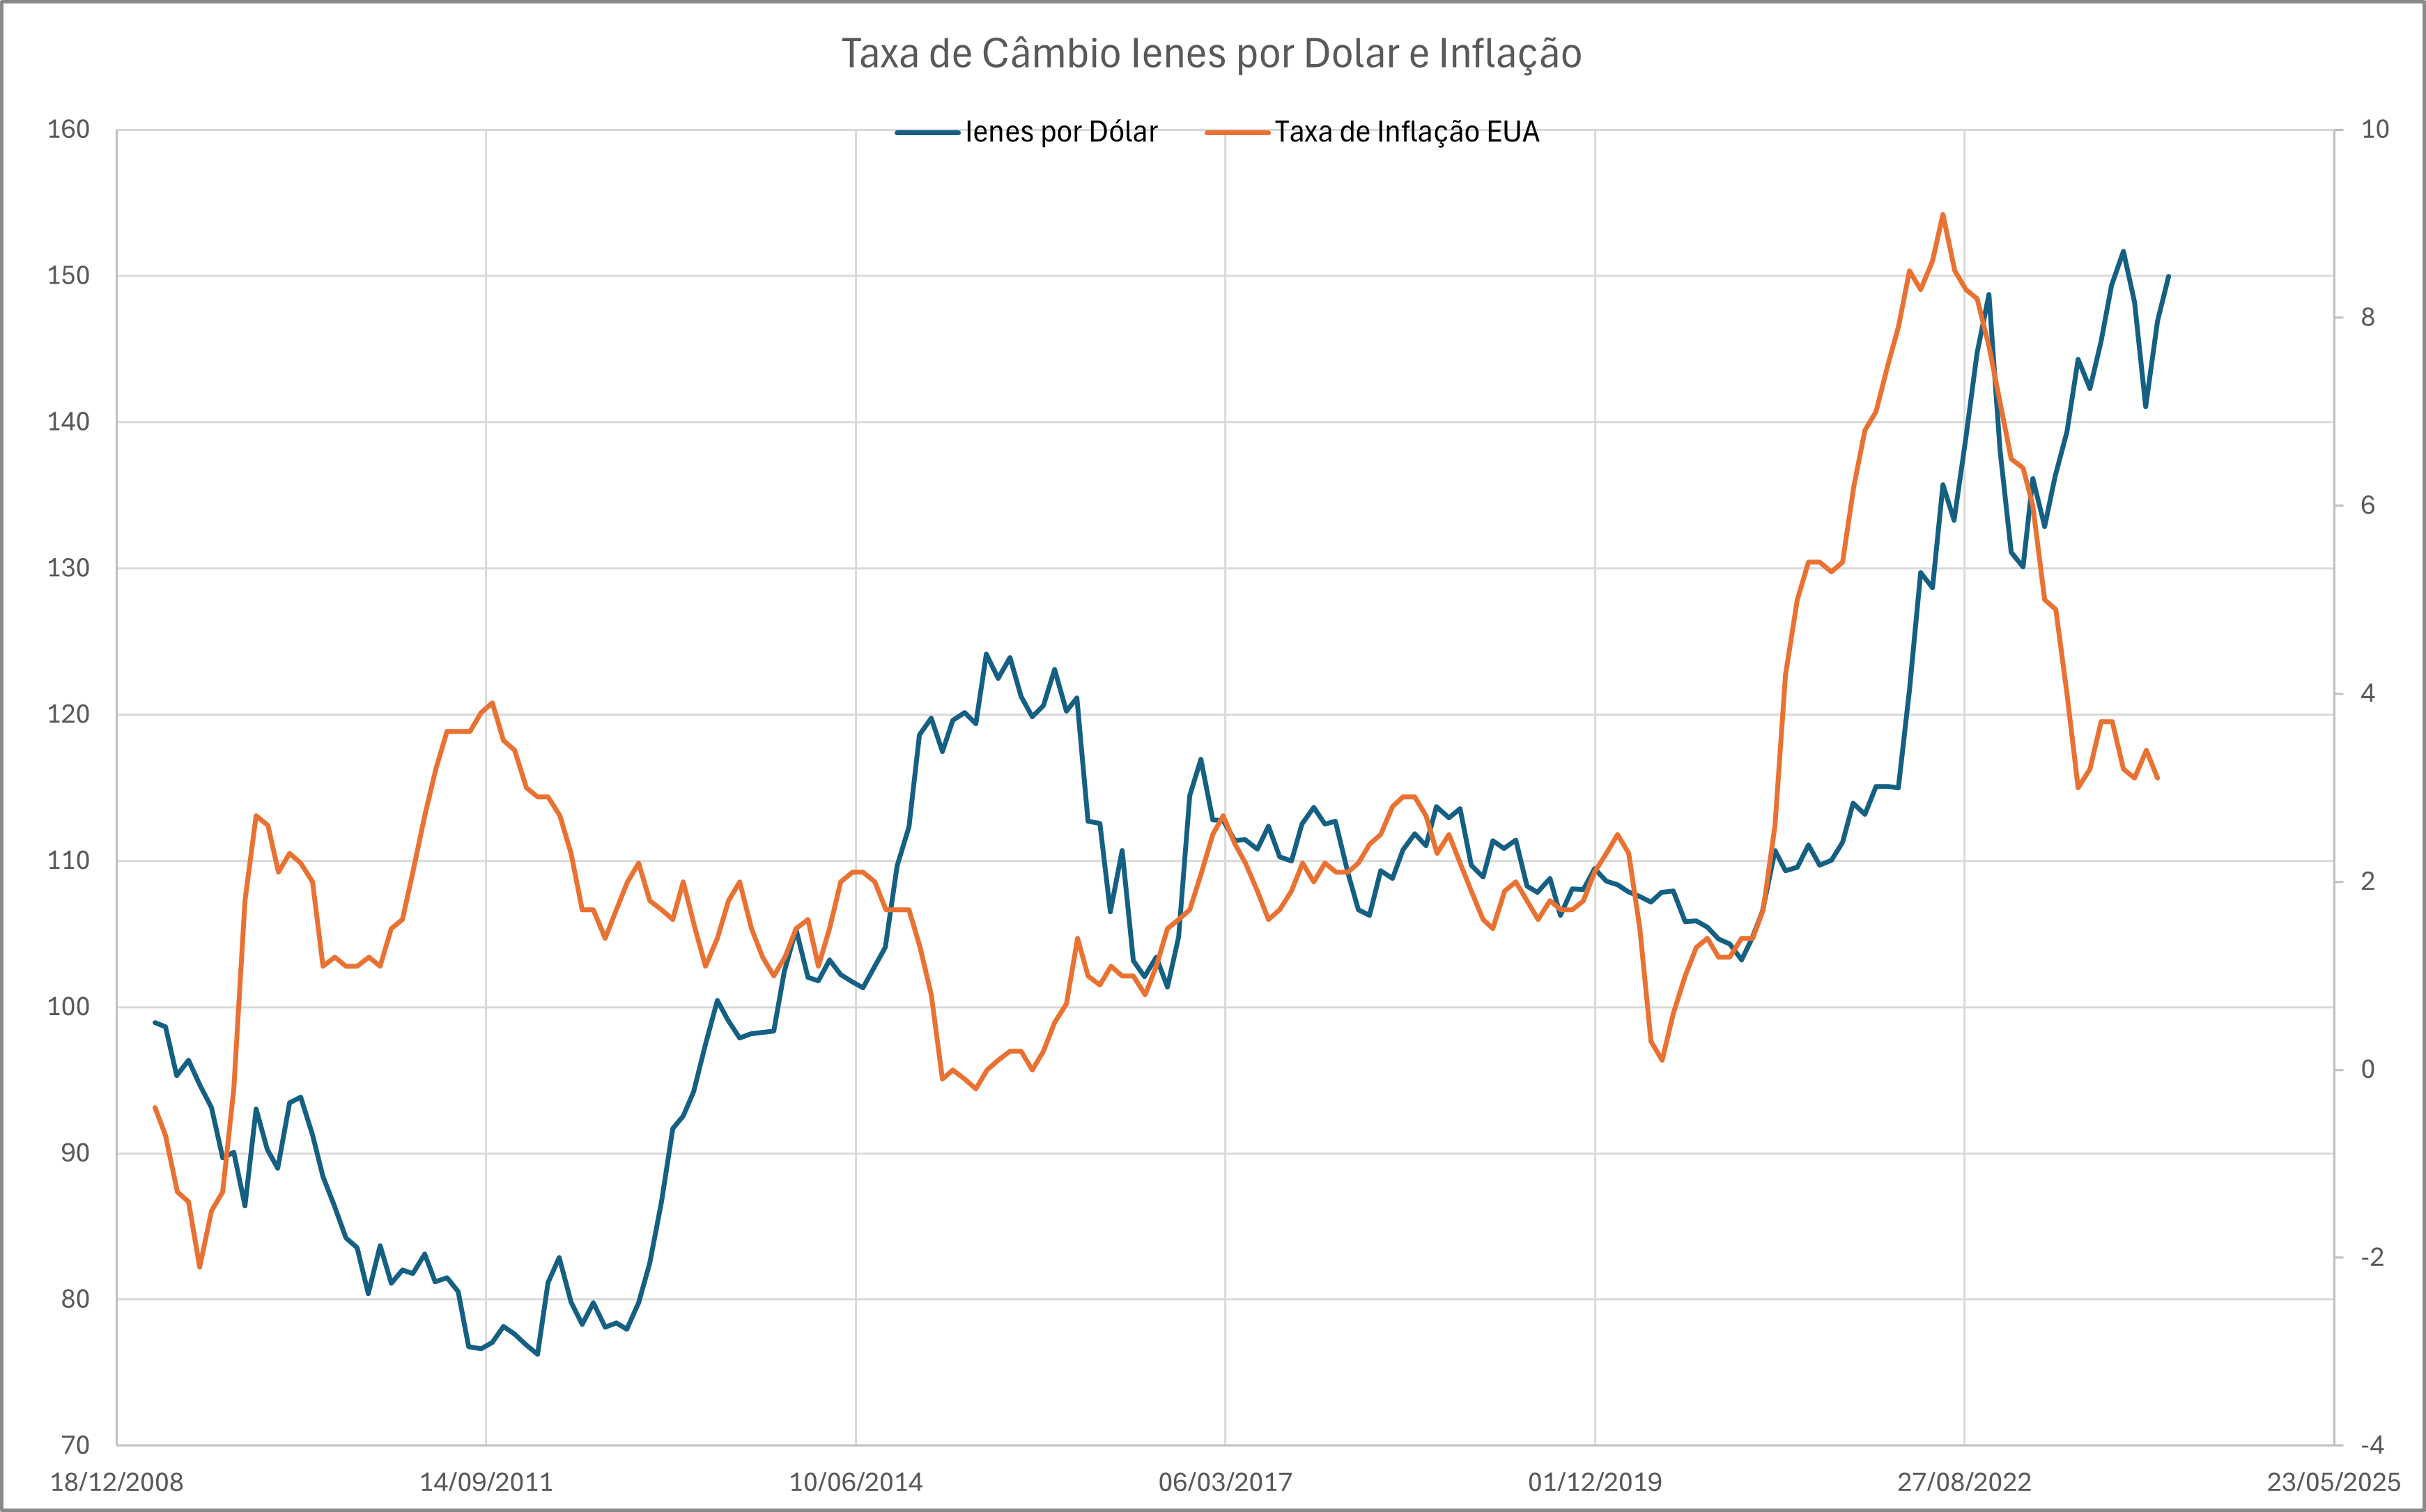
\includegraphics[width=0.75\textwidth]{Câmbio e Inflação estadunidense.png}
    \label{fig:cambioInflacaoEUA}
    
    \footnotesize{Fonte: Elaborado pelos autores.}
    \end{figure}

Intuitivamente, a desvalorização do dólar, provocada pela inflação, resulta em uma apreciação cambial, evidenciada pelo fortalecimento do iene. Isso é impulsionado pelo aumento da demanda pela moeda local.

\subsection{\textbf{Relação do Câmbio com os PIB's}}

O PIB de um país é um indicador que apresenta relação com o valor da moeda. Quando o PIB de um país está alto, significa que sua economia está aquecida, atraindo capital externo para ele. Assim, sua moeda se valoriza em relação a outras moedas (EUA nesse caso). No caso da relação entre o câmbio ienes por dólar (E) com o crescimento do PIB japonês, podemos ver a Figura~\ref{fig:cambioPIBJapão}.

\begin{figure}[H]
    \centering
    \caption{Gráfico da Taxa de Câmbio Iene por Dólar e PIB Japonês} 
    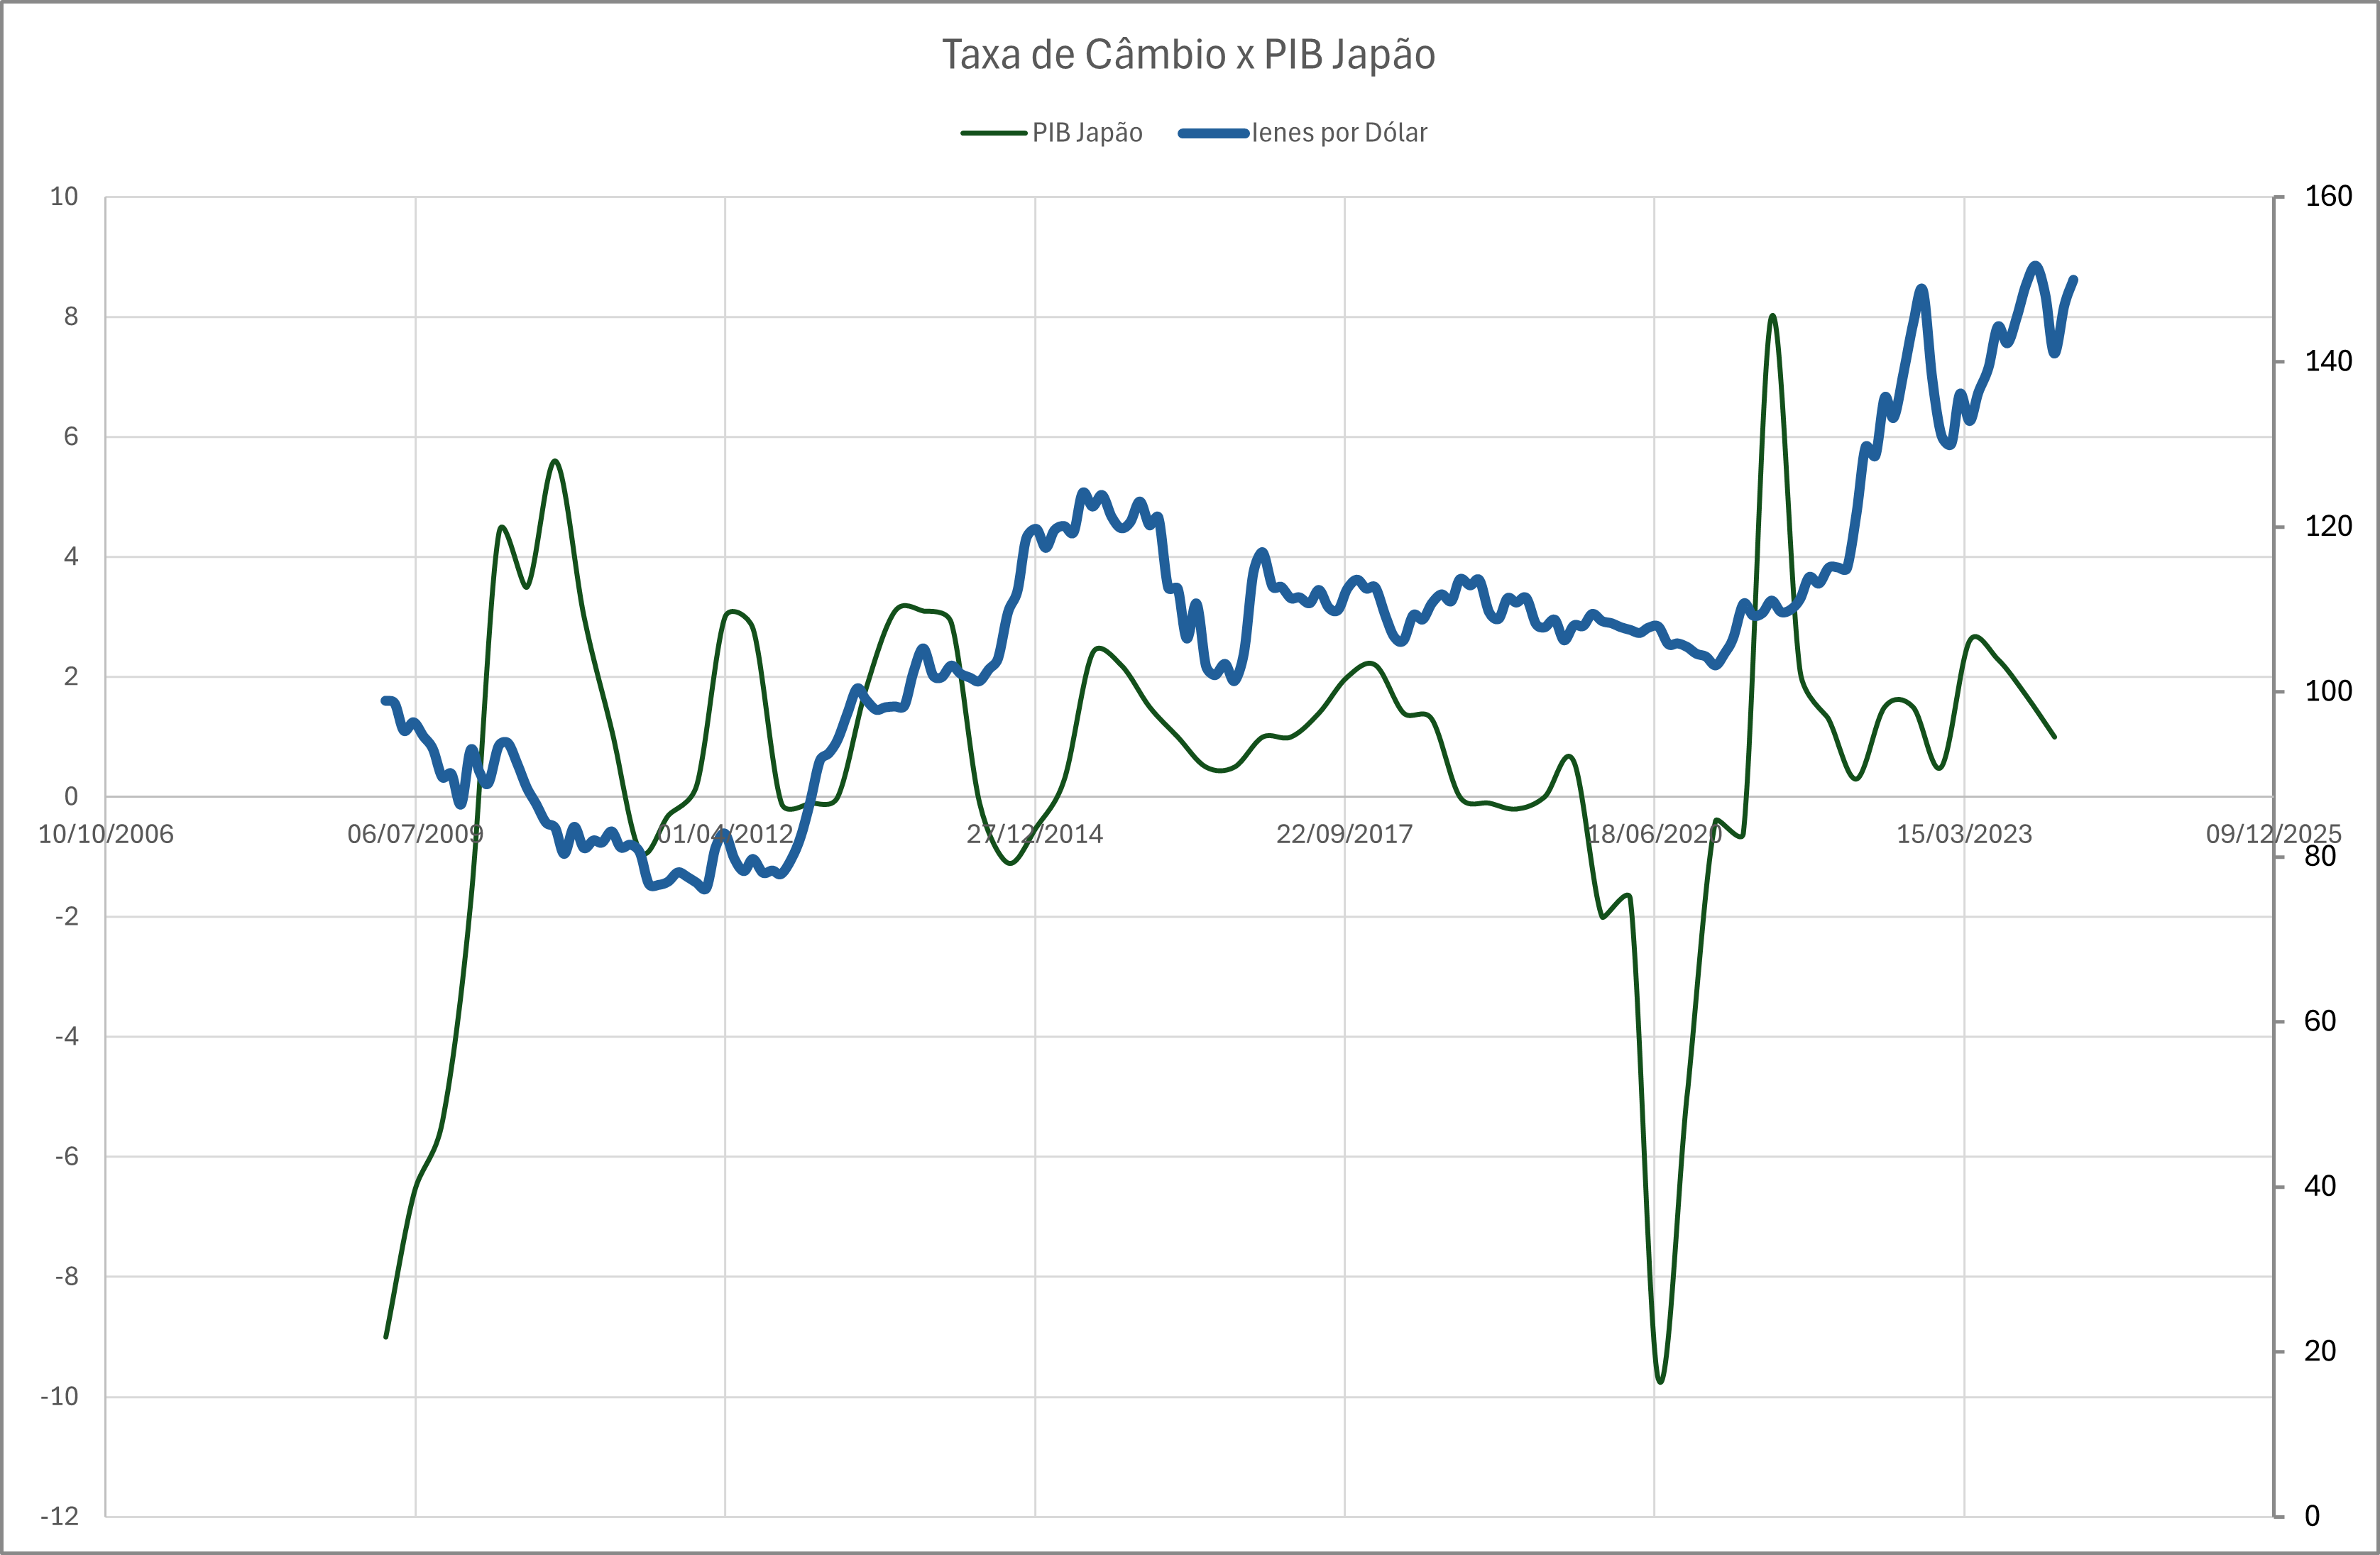
\includegraphics[width=0.75\textwidth]{PIB Japão.png}
    \label{fig:cambioPIBJapão}
    
    \footnotesize{Fonte: Elaborado pelos autores.}
    \end{figure}

No segundo semestre de 2014, por exemplo, houve decrescimento do PIB e concomitantemente depreciação do Iene em paridade ao Dólar. Vale ressaltar que as variáveis escolhidas não têm correlação perfeita com o movimento do câmbio e esse acontece a partir da relação do que acontece não apenas no Japão e EUA, como no resto do mundo. Isso pode ser visto na Figura~\ref{fig:cambioPIBEUA} abaixo. 

\begin{figure}[H]
    \centering
    \caption{Gráfico da Taxa de Câmbio Iene por Dólar e PIB Estadunidense} 
    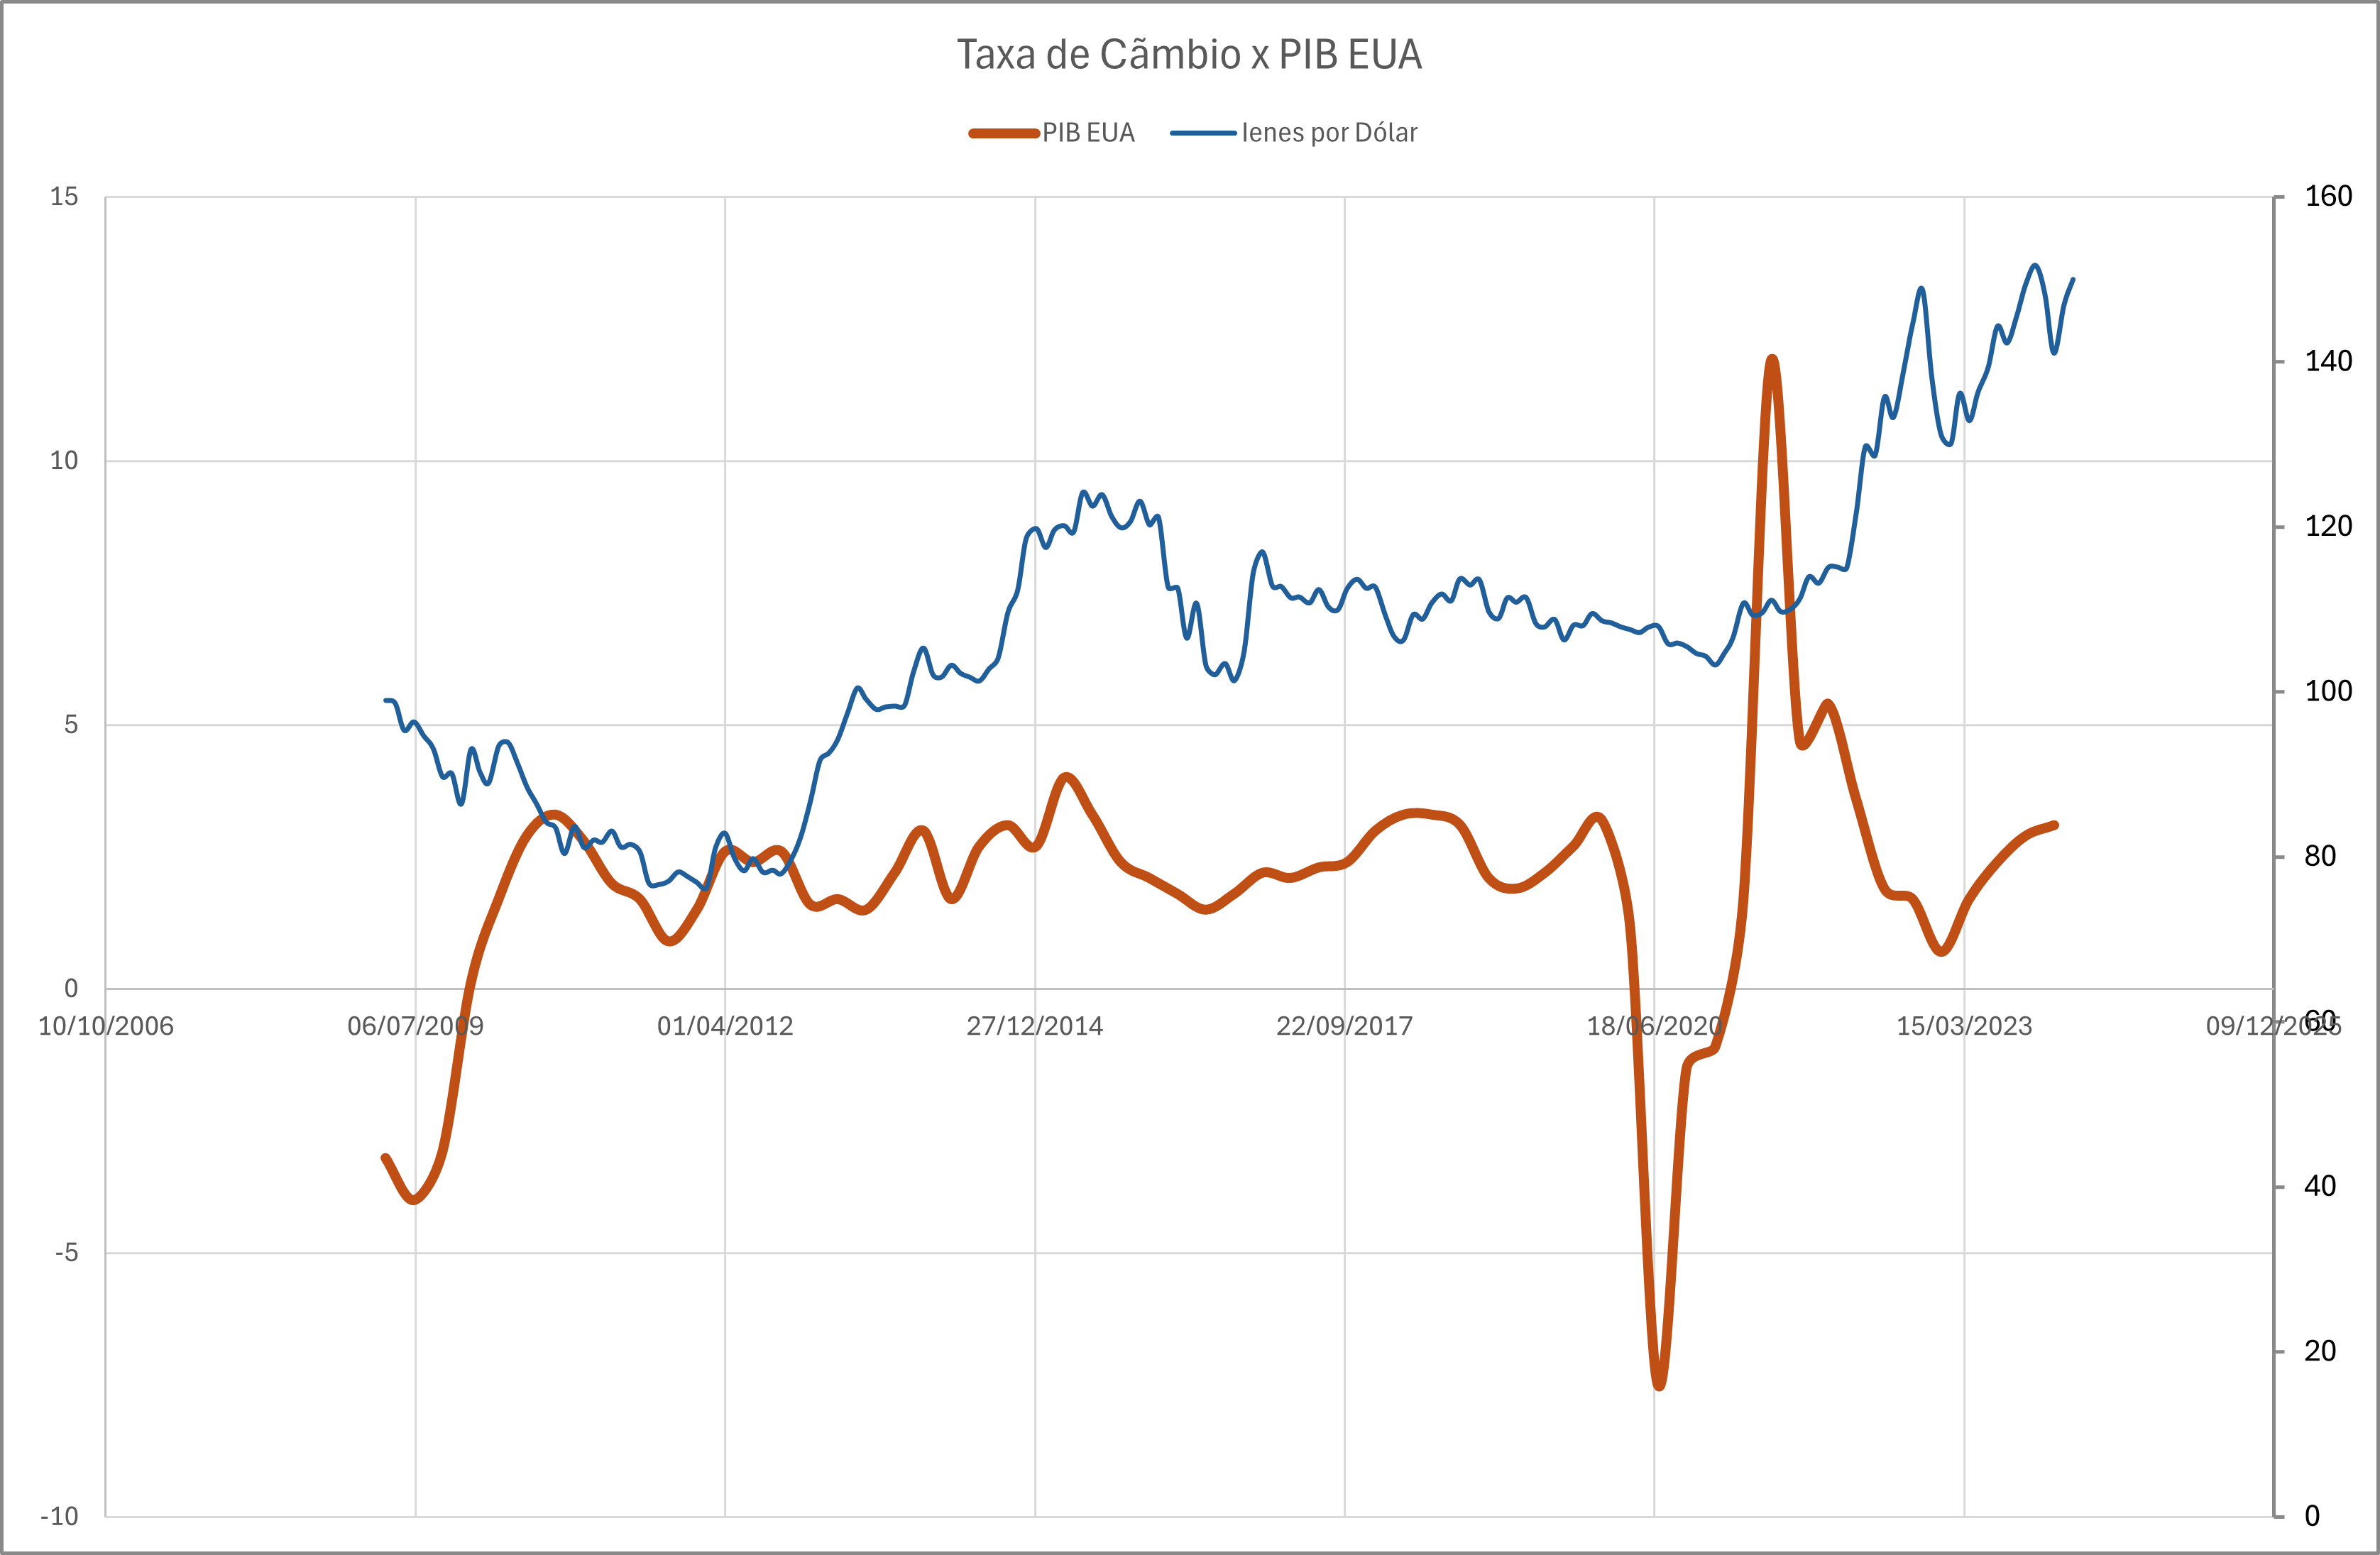
\includegraphics[width=0.75\textwidth]{PIB EUA.png}
    \label{fig:cambioPIBEUA}
    
    \footnotesize{Fonte: Elaborado pelos autores.}
    \end{figure}

No período da pandemia do COVID-19, por exemplo, os PIBs do EUA e do Japão tiveram decrescimento e mesmo assim suas taxas de câmbio não sofreram grandes alterações. Nesse cenário, grande parte das economias mundiais sofreram defasagem no crescimento, portanto, as moedas do EUA e do Japão não perderam tanta confiança em relação às outras.  

\subsection{\textbf{Conclusão Sobre a Previsão do Câmbio}}
As variáveis analisadas, apesar de possuírem uma alta relação com a intuição econômica das movimentações com a taxa de câmbio, têm impacto fundamental nele quando analisadas conjuntamente.

Ao realizar o processo da intuição econômica, fazemos o uso da estática comparativa, onde mexemos em uma variável e vemos o efeito na outro, apesar de ser um processo lógico correto, no mundo real mais de uma variável é responsável pela precificação do câmbio. Além disso, existem fatores que não são possíveis de "cravar" o exato valor, como a expectativa do valor de câmbio, que é um outro fator que contribui para a oscilação do câmbio.

\section{\textbf{Questão 3}}
\subsection{\textbf{Valorização do Iene , Ótica doméstica ; Japão}}
Para que o iene ganhe força em relação ao dólar, é necessário que haja fatores internos que aumentem a demanda por iene. Isso resultaria em uma valorização da moeda e, consequentemente, uma valorização da taxa de câmbio.

As variáveis que contribuem para a valorização da taxa de câmbio incluem um aumento no Produto Interno Bruto (PIB) e na taxa de juros, além de uma diminuição na taxa de inflação e na oferta monetária. Esses movimentos, de acordo com a lógica econômica, levam a uma valorização do iene e, consequentemente, a uma valorização da taxa de câmbio.

\subsection{\textbf{Valorização do Iene , Ótica externa ; Estados Unidos}}
Para que o iene ganhe força em relação ao dólar, é necessário que haja fatores externos que aumentem a oferta de dólar. Isso resultaria em uma desvalorização da moeda e, consequentemente, uma apreciação da taxa de câmbio.

As variáveis que contribuem para a valorização da taxa de câmbio incluem um redução no Produto Interno Bruto (PIB) e na taxa de juros, além de um aumento na taxa de inflação e na oferta monetária. Esses movimentos, de acordo com a lógica econômica, levam a uma desvalorização do dólar e, consequentemente, a uma valorização da taxa de câmbio.

\end{document}